\def\year{2015}
%File: formatting-instruction.tex
\documentclass{aamas2016}
\usepackage{color}
\usepackage{algorithm}
\usepackage{algorithmic}
\usepackage{wrapfig}
\frenchspacing
%\setlength{\pdfpagewidth}{8.5in}
%\setlength{\pdfpageheight}{11in}
\setcounter{secnumdepth}{2}
\usepackage{amsmath}  
\usepackage{amsfonts}
\DeclareMathOperator*{\argmin}{\arg\!\min} 
\DeclareMathOperator*{\argmax}{\arg\!\max} 
\usepackage{graphicx}
\usepackage{mathtools}
\usepackage{subcaption}
\DeclareGraphicsExtensions{.pdf,.png,.jpg}
\usepackage{subcaption}
\usepackage{hyperref}
\newif\ifnotes

%\usepackage{natbib}

%---------Toggle these flags if you want to supress the comments------------
\notestrue
%\notesfalse
%-----------------------------------------------------------------------------
\clubpenalty=10000 
\widowpenalty = 10000
\newcommand{\citet}[1]{\citeauthor{#1}~(\citeyear{#1})}
\definecolor{dark_green}{RGB}{46,200,50}
\definecolor{dim_gray}{RGB}{45,45,125}

\ifnotes

\pdfpagewidth=8.5truein
\pdfpageheight=11truein

 \begin{document}
% The file aaai.sty is the style file for AAAI Press 
% proceedings, working notes, and technical reports.
%
\title{Inverse Reinforcement Learning from Failure}

% AUTHORS


% For initial submission, do not give author names, but the
% tracking number, instead, as the review process is blind.

% You need the command \numberofauthors to handle the 'placement
% and alignment' of the authors beneath the title.
%
% For aesthetic reasons, we recommend 'three authors at a time'
% i.e. three 'name/affiliation blocks' be placed beneath the title.
%
% NOTE: You are NOT restricted in how many 'rows' of
% "name/affiliations" may appear. We just ask that you restrict
% the number of 'columns' to three.
%
% Because of the available 'opening page real-estate'
% we ask you to refrain from putting more than six authors
% (two rows with three columns) beneath the article title.
% More than six makes the first-page appear very cluttered indeed.
%
% Use the \alignauthor commands to handle the names
% and affiliations for an 'aesthetic maximum' of six authors.
% Add names, affiliations, addresses for
% the seventh etc. author(s) as the argument for the
% \additionalauthors command.
% These 'additional authors' will be output/set for you
% without further effort on your part as the last section in
% the body of your article BEFORE References or any Appendices.

%\numberofauthors{8} %  in this sample file, there are a *total*
% of EIGHT authors. SIX appear on the 'first-page' (for formatting
% reasons) and the remaining two appear in the \additionalauthors section.
%

\numberofauthors{3}

\author{
% You can go ahead and credit any number of authors here,
% e.g. one 'row of three' or two rows (consisting of one row of three
% and a second row of one, two or three).
%
% The command \alignauthor (no curly braces needed) should
% precede each author name, affiliation/snail-mail address and
% e-mail address. Additionally, tag each line of
% affiliation/address with \affaddr, and tag the
% e-mail address with \email.
% 1st. author
\alignauthor
Kyriacos Shiarlis\\
       \affaddr{Informatics Institute}\\
       \affaddr{University of Amsterdam}\\
       \affaddr{Science Park 904}\\
       \affaddr{Amsterdam, Netherlands}\\
       \email{k.c.shiarlis@uva.nl}
\alignauthor
Joao Messias\\
       \affaddr{Informatics Institute}\\
       \affaddr{University of Amsterdam}\\
       \affaddr{Science Park 904}\\
       \affaddr{Amsterdam, Netherlands}\\
       \email{j.messias@uva.nl}
\alignauthor
Shimon Whiteson\\
       \affaddr{Dept.\ of Computer Science}\\
       \affaddr{University of Oxford}\\
       \affaddr{Wolfson Building, Parks Rd}\\
       \affaddr{Oxford, United Kingdom}\\
       \email{shimon.whiteson@cs.ox.ac.uk}
}

% Association for the Advancement of Artificial Intelligence\\
% 2275 East Bayshore Road, Suite 160\\
% Palo Alto, California 94303\\
% }
\maketitle
\begin{abstract}

\emph{Inverse reinforcement learning} (IRL) allows autonomous a\-gents to learn to solve complex tasks from successful demonstrations.  However, in many settings, e.g., when a human learns the task by trial and error, \emph{failed} demonstrations are also readily available.  In addition, in some tasks, purposely generating failed demonstrations may be easier than generating successful ones.  Since existing IRL methods cannot make use of failed demonstrations, in this paper we propose \emph{inverse reinforcement learning from failure} (IRLF) which exploits both successful and failed demonstrations.  Starting from the state-of-the-art \emph{maximum causal entropy IRL} method, we propose a new constrained optimisation formulation that accommodates both types of demonstrations while remaining convex.  We then derive update rules for learning reward functions and policies. Experiments on both simulated and real-robot data demonstrate that IRLF converges faster and generalises better than maximum causal entropy IRL, especially when few successful demonstrations are available.
\end{abstract}

\category {I.2.6}{Artifficial Intelligence}{Learning}
%A category including the fourth, optional field follows...
%\category{D.2.8}{Software Engineering}{Metrics}[complexity measures, performance measures]

%General terms should be selected from the following 16 terms: Algorithms, Management, Measurement, Documentation, Performance, Design, Economics, Reliability, Experimentation, Security, Human Factors, Standardization, Languages, Theory, Legal Aspects, Verification.

\terms{Algorithms}

%Keywords are your own choice of terms you would like the paper to be indexed by.

\keywords{Inverse reinforcement learning, learning from demonstration, social navigation, robotics, machine learning.}

\section{Introduction}

In \emph{inverse reinforcement learning} (IRL) \cite{ng2000algorithms}, an \emph{apprentice} aims to learn a policy for acting in an environment, typically modelled as a \emph{Markov decision process} (MDP), for which the reward function is not available, but successful demonstrations provided by an \emph{expert} performing the task are given instead. An IRL algorithm tries to find a reward function that leads the apprentice to behave  similarly to the expert while generalising well to situations for which expert data is not available. 

%Numerous IRL methods have been developed, using structured prediction \cite{klein2012inverse,ratliff2006maximum}, Bayes\-ian inference \cite{ramachandran2007bayesian}, Gaussian processes \cite{levine2011nonlinear}, and decision trees \cite{ratliff2007boosting} to learn reward functions. IRL has been applied to many tasks, e.g., simulated car driving \cite{abbeel2004apprenticeship}, learning autonomous driving styles \cite{kuderer2015learning} and socially appropriate navigation \cite{henry2010learning,vasquez2014inverse}. 

Numerous IRL methods have been proposed. In \cite{ratliff2006maximum} a structured prediction formulation using maximum margin is developed and applied to mobile robotics. In \cite{ramachandran2007bayesian},  a  Bayesian formulation is proposed along with approximations necessary for computational tractability. Other work considers nonlinear representations of the reward function using Gaussian processes \cite{levine2011nonlinear} or decision trees \cite{ratliff2007boosting}. IRL has also been applied to a wide range of applications, from  autonomous driving \cite{abbeel2004apprenticeship,kuderer2015learning} to socially appropriate navigation \cite{henry2010learning,vasquez2014inverse} and training parsers for natural language processing \cite{neu2009training}.


Existing IRL algorithms learn only from successful demonstrations, i.e., from data gathered by an expert performing the task well. This is consistent with the main motivation of IRL since it allows learning in tasks where the reward cannot be trivially hard-coded.  For example, the reward function that allows an agent to perform complicated manoeuvres while flying a helicopter cannot be trivially determined, but example demonstrations are easy to obtain from an expert.

In many realistic scenarios, failed demonstrations are also readily available.  Consider for example tasks such as driving a car.  Since humans also learn this task by trial and error, demonstrations of both successful and failed behaviour are available. Although hand-coding a reward function for this task would be infeasible, labelling each trial as successful or failed is straightforward.  
In addition, in many tasks, it may be easier to demonstrate failure than success.  If expert demonstrations are scarce but a safe simulator is available, a non-expert can often easily demonstrate multiple failure modes, yielding data that complements the scarce successful demonstrations. This idea is explored in \cite{choi2015}, where a robot learns to avoid people using simulations of failed avoidance. Finally, failed demonstrations may be used to explore the state-action space, an idea previously leveraged in learning from demonstration \cite{grollman2011donut}.

In existing IRL methods, failed demonstrations have been treated as noise \cite{zheng2014robust} and filtered out in order to improve robustness. However, such methods do not actually use such demonstrations for learning.

In this paper, we introduce \emph{inverse reinforcement learning from failure} (IRLF), which is to our knowledge the first IRL algorithm that can learn from both successful and failed demonstrations. In doing so, we address a key difficulty in IRL: the problem is typically under-constrained since many reward functions are consistent with the expert's behaviour.  By exploiting failed demonstrations, our method reduces this ambiguity, resulting in faster and better learning.

To derive IRLF, we start from the state-of-the-art \emph{maximum causal entropy IRL} \cite{ziebart2008maximum,ziebart2010modelingthesis} method, which is also related to \cite{babes2011apprenticeship}. We propose a new constrained optimisation formulation that accommodates both successful and failed demonstrations while remaining convex.  We then derive update rules for learning policies and reward functions.

We evaluate our algorithm on the task of social navigation for a mobile robot, using both simulated and real-robot data, as well as the \emph{Factory} problem, a well known decision making benchmark. On the simulated scenarios, our results demonstrate that IRLF generalises better than maximum causal entropy IRL when successful demonstrations are scarce, with little additional computational cost.  On the real-robot data, IRLF also outperforms this baseline. 

% \jm{I omitted an argument that the algorithm is able to learn ``mixtures of behaviors'' from successful and failed examples, since that is quite difficult to fit in here without raising too much confusion} 


\section{Background}
Most IRL methods formalise the underlying decision-mak\-ing problem as a \emph{Markov decision process} (MDP), a model of a discrete-time process wherein an agent's actions may stochastically influence its environment. In an MDP, at step $t$, the system (which includes the agent and its environment) is known to be in a \emph{state} $s_t\in\mathcal{S}$; the agent selects an action $a_t\in\mathcal{A}$ and is awarded a real-valued \emph{reward}; and the system jumps to state $s_{t+1}$ with probability $P(s_{t+1}|s_t,a_t)$. Formally, an MDP is a tuple $\langle\mathcal{S},\mathcal{A},T,R\rangle$, where $\mathcal{S}$ and $\mathcal{A}$ are sets of discrete states and actions respectively, $T:\mathcal{S}\times\mathcal{A}\times\mathcal{S}\rightarrow [0,1]$ is a transition function such that $T(s,a,s')=P(s'|s,a)$, and $R:\mathcal{S}\times\mathcal{A}\rightarrow\mathbb R$ is the reward function. 
Optimally solving an MDP involves finding a policy $\pi:\mathcal{S}\times\mathcal{A}\rightarrow[0,1]$ with $\pi(s,a) = P(a\,|\,s)$, that maximises the expected sum of rewards over a fixed number of decisions $h$. This expectation can be expressed as the \emph{value} of policy $\pi$:
\begin{equation}
\label{eq:value}
 V^\pi(s) \coloneqq E\{\sum_{t = 1}^hR(s_t,a_t)\,\vert\, s_1 = s\}.
\end{equation}

Given data obtained from interacting with an MDP, RL methods seek a policy that maximises this expectation for a given reward function.  By contrast, given data obtained from \emph{expert} interactions with an MDP, IRL seeks the reward function that the expert was maximising.  IRL is useful in the many situations in which the expert cannot easily formalize her objectives as a reward function.  Instead, the \emph{learner}, an autonomous agent, can learn the reward function from the expert's behaviour and use it to imitate her.

IRL is formalised as an `incomplete' MDP $\langle\mathcal{S},\mathcal{A},T\rangle$, also known as an MDP/R. Though initially unknown, the reward function is parametrised by $K$ \emph{feature functions}, $\phi_k(s,a)$:
\begin{equation}
R(s,a) = \sum_{k=1}^Kw_k\phi_k(s,a), \label{eq:rew}
\end{equation}
where $w=[w_1\,w_2\,\ldots\,w_k]^T$ is the weight vector that IRL aims to learn.

Since $w$ is independent of states and actions, \eqref{eq:value} and \eqref{eq:rew} imply a parametric form of the value function:
\begin{align}
 	V^{\pi}(s) &= \sum^K_{k=1}w_k\left(E\{\sum_{t = 1}^h\phi_k(s_t,a_t)\,\vert\, s_1 = s\}\right)\\
&\eqqcolon\sum^K_{k=1}w_k\mu^{\pi, 1:h}_k|_{s_1=s},\label{eq:parametrized_value}
\end{align}
where $\mu^{\pi,1:h}_k|_{s_1=s}$, the \emph{feature expectation}, is the expected accumulation of instances of feature $\phi_k$ between steps $1$ and $h$ under policy $\pi$  given that $s_1 = s$. The step indices are omitted for simplicity when this expectation is over the full horizon $\{1,\ldots,h\}$.

The learner learns from a dataset of $N$ trajectories, $\mathcal{D} = \big\{ \tau_1,\tau_2,...\tau_N \big\}$. Each trajectory $\tau_i~=~\langle(s^{\tau_i}_1,a^{\tau_i}_1),(s^{\tau_i}_2,a^{\tau_i}_2),$ $\ldots,(s^{\tau_i}_{h},a^{\tau_i}_{h})\rangle$ is a state-action sequence of length $h$ generated by the expert.
Given $\mathcal{D}$, the learner can compute the \emph{empirical feature expectation}, the average accumulated instances of each feature in $\mathcal{D}$:
\begin{equation}
	\widetilde{\mu}^{\mathcal{D}}_k \coloneqq\frac{1}{N}\sum_{\tau\in\mathcal{D}}\sum_{t=1}^{h}\phi_k(s^\tau_t,a^\tau_t). \label{eqn:empirical_fe}
\end{equation}
Note that $\widetilde{\mu}^{\mathcal{D}}_k$ is state independent and implicitly estimates an expectation across
the expert's initial state.  To fairly compare the feature expectation of some policy $\pi$ to $\widetilde{\mu}^{\mathcal{D}}_k$, we obtain an analogously state-independent measure of $\pi$'s feature expectation by marginalising out $s_1$:
\begin{align}
  \label{eq:feature_expectation_belief}
  \mu^{\pi}_k|_{\mathcal{D}} \coloneqq \sum_{s\in\mathcal{S}}P_{\mathcal{D}}(s_1 = s)\mu^{\pi}_k|_{s_1=s},
\end{align}
where $P_{\mathcal{D}}(s_1 = s)= N_1(s)/N$ is the maximum likelihood estimate of the expert's initial state distribution, given that $N_1(s)$ is the number of trajectories with $s_1 = s$.

The learner aims to find $w$ such that the distance between the vectors $\widetilde\mu^{\mathcal{D}}~=~[\widetilde\mu^{\mathcal{D}}_1\,\ldots\,\widetilde\mu^{\mathcal{D}}_k]^T$ and $\mu^{\pi}|_{\mathcal{D}}~=~[\mu^{\pi}_1|_{\mathcal{D}}\,\ldots\,\mu^{\pi}_k|_{\mathcal{D}}]$ is minimised according to some metric, while also generalising well to unseen initial conditions.

IRL methods are typically iterative. An initial guess for $w$ is fed to a planner that produces a policy $\pi$ that is optimal given $w$.  Using $\pi$, trajectories are generated from the same initial states as in $\mathcal{D}$ to compute $\mu^{\pi}|_{\mathcal{D}}$, which is then compared to $\widetilde{\mu}^{\mathcal{D}}$.  Finally, $w$ is updated to reduce to distance between the two expectations, and the process repeats.

The task  of finding $w$ can be formulated as an optimisation problem that requires the expert trajectories to have maximal value \cite{abbeel2004apprenticeship} or that do so by some margin \cite{ratliff2006maximum}. Alternatievely one may employ Bayesian inference \cite{ramachandran2007bayesian,dimitrakakis2012bayesian} to compute a posterior distribution over the weights.  In this paper, we concentrate on methods that learn maximum-entropy policies \cite{ziebart2008maximum,ziebart2010modelingthesis}.  A maximum-entropy approach is attractive because it is probabilistic and thus robust to noise and randomness in the actions of the expert, and results in convex optimisation problems. The methods work by solving the following constrained optimisation problem:
\begin{align}
	\hbox{find:} &\quad\max\limits_{\pi} H(\mathcal{A}^h||\mathcal{S}^h)\label{eq:primal_obj}\\
\hbox{subject to:}&\quad\widetilde{\mu}^{\mathcal{D}}_k   = \mu^{\pi}_k|_{\mathcal{D}}\quad\forall k \label{eq:features_equality_constraint}\\
\hbox{and:} &\quad\sum_{a\in\mathcal{A}}\pi(s,a)  = 1\quad\forall s\in\mathcal{S}\\
\hbox{and:} &\quad\pi(s,a) \geq 0\quad\forall s\in\mathcal{S},a\in\mathcal{A},\label{eq:positive_policy}
\end{align}
where $H(\mathcal{A}^h||\mathcal{S}^h)$, the \emph{causal entropy}, is the conditional entropy of the action sequence $\mathcal{A}^h$, causally conditioned on the state sequence $\mathcal{S}^h$:
% For MDPs this quantity is fully determined given a policy $\pi$ and a transition function $T$:
\begin{align}
H(\mathcal{A}^h||\mathcal{S}^h) = -\sum_{t=1}^h \sum_{\substack{s_{1:t}\in\mathcal{S}^t\\a_{1:t}\in\mathcal{A}^t}} P(a_{1:t},s_{1:t})\log(P(a_t|s_t)),
\label{eg:entdef}
\end{align}
where:
\begin{align*}
  P(a_{1:t},s_{1:t})&= P(s_{1:t-1},a_{1:t-1})P(s_t|s_{t-1},a_{t-1})P(a_t|s_t)\\
  &=P(s_{1:t-1},a_{1:t-1})T(s_{t-1},a_{t-1},s_t)\pi(s_t,a_t).
\end{align*}
The constraints require that $\pi$ consists of proper probability distributions that match the empirical feature expectations.

The optimisation problem is solved using the method of Lagrange multipliers. First, the equality constraint \eqref{eq:features_equality_constraint} is relaxed, yielding a Lagrangian:
\begin{equation}
\label{eq:partial_lagrangian}
\mathcal{L}(\pi,w)\coloneqq H(\mathcal{A}^h||\mathcal{S}^h) + \sum_{k=1}^Kw_k(\mu^{\pi}_k|_{\mathcal{D}}-\widetilde{\mu}^{\mathcal{D}}_k),
\end{equation}
and in turn a less constrained optimisation problem:
\begin{align}
\hbox{find:}\,\,&\,\,\min_{w}\left\{\max_\pi\left(\mathcal{L}(\pi,w)\right)\right\}\label{eq:partial_dual_obj}\\
\hbox{subject to:}\,\,&\sum_{a\in\mathcal{A}}\pi(s,a)  = 1\quad\forall s\in\mathcal{S}\label{eq:dual_constraint_1}\\
\hbox{and:}\,\,&\pi(s,a) \geq 0\quad\forall s\in\mathcal{S},a\in\mathcal{A},\label{eq:dual_constraint_2}
\end{align}

Differentiating $\mathcal{L}(\pi,w)$ with respect to $\pi$ at time $t$ results in \cite[p.\ 186]{ziebart2010modelingthesis}:
\begin{equation}
 \begin{split}
 &\nabla_{\pi(s_t,a_t)}\mathcal{L}(\pi,w) = P(s_{1:t},a_{1:t-1})\Bigg(-\log(\pi(a_t,s_t))+ \\
& H(\mathcal{A}^{t+1:h}||\mathcal{S}^{t+1:h})
 +\sum_{k=1}^K w_kE\left\{\sum_{\tau=1}^h \phi_k(s_t,a_t)|s_{1:t},a_{1:t-1}\right\}\Bigg). \label{eqn:zieb_lagragian_derivative}
 \end{split}
\end{equation}
Setting the gradient to zero and solving for $\pi$ gives:
\begin{equation}
\label{eq:policy_prop}
	\begin{split}
	&\pi(s_t,a_t) \propto \exp\left(H(\mathcal{A}^{t:h}||\mathcal{S}^{t:h})+\sum^K_{k=1} w_k\mu_k^{\pi,t:h}|_{s_t,a_t}\right).
	\end{split}
\end{equation}
Due to \eqref{eq:parametrized_value}, the rightmost term in \eqref{eq:policy_prop} is a measure of value for a given state and action, parametrised by $w$. \cite{ziebart2010modelingthesis} showed that solving \eqref{eq:policy_prop} while satisfying \eqref{eq:dual_constraint_1} and \eqref{eq:dual_constraint_2} amounts to solving a soft Bellman equation:
	\begin{equation}
		\begin{split}
	&Q_w(s,a)^{soft} = \sum_{k=1}^Kw_k\phi_k(s,a) + \sum_{s'}T(s,a,s')V_w(s'),\\	
	&V_w(s)^{soft} = \log\sum_{a}exp(Q_w(s,a)),\\
	&\pi(s,a) = \exp(Q_w(s,a) - V_w(s)).
	\end{split}
	\label{eq:soft_backup}
	\end{equation}
Once $\pi$ is computed for a given $w$, $w$ is updated via gradient descent, by noting that:
 \begin{align}
   \label{eq:weight_update}
   \nabla_{w}\mathcal{L}(\pi,w) =\mu^\pi|_{\mathcal{D}} - \mu^{\mathcal{D}},
 \end{align}
where $\mu^\pi|_{\mathcal{D}}$ is computed by rolling out policy $\pi$ from the initial state distribution $P_{\mathcal{D}}(s_1)$ over $h$ steps, and taking an expectation over the features accumulated at each step. The optimisation process terminates once the weight vector converges to the optimal solution.

\section{Method}
In this section, we propose \emph{inverse reinforcement learning from failure} (IRLF), a novel IRL algorithm that exploits failed demonstrations.  IRLF is applicable in settings where the apprentice has access to a dataset $\mathcal{F}$ of failed demonstrations, in addition to a dataset $\mathcal{D}$ of successful ones.

A critical challenge in developing such a method is deciding how to interpret failed trajectories.  While successful trajectories may not be optimal, it is clear that the agent should try to imitate them, which in our case means matching feature expectations.  By contrast, a failed trajectory is more ambiguous because it is unclear what about it is wrong: was the entire trajectory incorrect, or was it almost correct but wrong with respect to one particular feature? A key characteristic of the method we propose is that it works well in both these cases.

%\aama{The first obstacle in doing so, is a semantic one. Successful demonstrations have a clear semantic meaning, they are in some sense optimal. Algorithms that learn from succesful demonstrations have the clear aim to match some description of these demonstrations (in our case, the feture expectations). On the other hand, failed demonstrations are semantically more ambiguous. For example a demonstration could be in its majority very well executed, but catastrophic as a whole. Another possibility is that we have access to demonstrations that can be considered failed, by a different degree. During our derivation and experiments we will repeateatly return to this semantic difference in order to show that IRLF deals with such ambiguities elegantly. }

The first step is to formulate a new constrained optimisation problem analogous to \eqref{eq:primal_obj}--\eqref{eq:positive_policy}. In addition to requiring that the feature expectations of the learned policy match the empirical expectations of $\mathcal{D}$, we now also want those feature expectations to be \emph{dissimilar} to the empirical expectations of $\mathcal{F}$. Although successful and failed demonstrations are semantic opposites, incorporating the latter into IRL proves to be nontrivial.

A straightforward approach is to add inequality constraints to the optimisation problem:
	\begin{equation}
        \label{eq:abs_inequality}
	|\widetilde{\mu}^{\mathcal{F}}_k  - \mu^{\pi}_k|_{\mathcal{F}}| > \alpha_k \quad\forall k,
	\end{equation} 
where $\widetilde{\mu}^{\mathcal{F}}_k$ is the empirical expectation of feature $k$ according to $\mathcal{F}$, computed analogously to \eqref{eqn:empirical_fe}, and $\alpha_k$ is a variable to be maximised as part of the optimisation objective, which becomes:
	\begin{equation}
		\quad\max\limits_{\pi,\alpha} H(\mathcal{A}^h||\mathcal{S}^h) + \sum^K_{k=1} \alpha_k.
	\end{equation}
However, this formulation is problematic because \eqref{eq:abs_inequality} is not a convex constraint. In fact, this approach is equivalent to maximising the $L_1$ norm of $\widetilde{\mu}^{\mathcal{F}}  - \mu^{\pi}|_{\mathcal{F}}$, which is nonconvex.

A convex relaxation of the above approach can be formulated by removing the extra constraint in \eqref{eq:abs_inequality} and instead adding to the objective the inner product of a parameter vector $\theta=\left[\theta_1~\ldots~\theta_k\right]^T$ and the difference in feature expectations, yielding the following objective function:
	\begin{equation}
		\max\limits_{\pi,\theta} H(\mathcal{A}^h||\mathcal{S}^h) + \sum^K_{k=1} \theta_k (\mu^{\pi}_k|_{\mathcal{F}} - \widetilde{\mu}^{\mathcal{F}}_k).
	\end{equation}
However, this approach is also problematic because it complicates the maximisation of the Lagrangian. We now need to find a critical point with respect to \emph{both} $\pi$ and $\theta$, which is analytically involved and numerically expensive, since it requires calculating $\mu^{\pi}|_{\mathcal{F}}$ each time that $\pi$ is updated via the soft Bellman backup in \eqref{eq:soft_backup}.

To avoid these difficulties, we propose a different formulation.  The main idea is to create new equality constraints of the form $\mu_k^{\pi}|_{\mathcal{F}} -\widetilde{\mu}_k^{\mathcal{F}}=z_k$ with $z_k\in\mathbb R$, and introduce the $z_k$ variables as terms in the optimisation objective.  The complete constrained optimisation problem is thus:
\begin{align}
 \quad\max\limits_{\pi,\theta,z}&\quad H(\mathcal{A}^h||\mathcal{S}^h) + \sum_{k=1}^K \theta_k z_k - \frac{\lambda}{2}||\mathbf{\theta}||^2 \label{eq:primal_obj_failure}\\
\hbox{subject to:}&\quad \quad\mu^{\pi}_k|_{\mathcal{D}}=\widetilde{\mu}^{\mathcal{D}}_k\quad\forall k \label{eq:features_equality_constraint_failure}\\
\hbox{and:}&\quad \quad  \mu_k^{\pi}|_{\mathcal{F}} -\widetilde{\mu}_k^{\mathcal{F}}=z_k \quad \forall k\\
\hbox{and:}&\quad \quad\sum_{a\in\mathcal{A}}\pi(s,a)  = 1\quad\forall s\in\mathcal{S}\\
\hbox{and:}&\quad \quad\pi(s,a) \geq 0\quad\forall s\in\mathcal{S},a\in\mathcal{A},  
\end{align}
where $\lambda$ is a constant.  
%\sw{It's standard to use $\lambda$ for the regularisation parameter.  If we use $\alpha$ for the learning rate later, which is also standard, there is no conflict.} \jm{fixed} 
Intuitively, the first term in the objective seeks to maximise $\pi$'s causal entropy, while the second term balances this against maximising dissimilarity between $\pi$'s feature expectations and the empirical expectations in $\mathcal{F}$; the third term regularises to discourage large values of $\theta$.

The main advantage of this formulation is that $\pi$ and $\theta$ become decoupled for a given $z$, making maximisation of the Lagrangian feasible while preserving convexity. 
%\sw{Is that right?} \jm{yes} 
Specifically, the new Lagrangian is:
\begin{equation}
\begin{split}
\label{eq:partial_lagrangian_failure}
\mathcal{L}(\pi,\theta,z &,w^{\mathcal{D}},w^{\mathcal{F}})=  H(\mathcal{A}^h||\mathcal{S}^h) - \frac{\lambda}{2}||\theta||^2 + \sum_{k=1}^K\theta_kz_k+\\
&
\sum_{k=1}^Kw^{\mathcal{D}}_k(\mu^{\pi}_k|_{\mathcal{D}}-\widetilde{\mu}^{\mathcal{D}}_k) + 
\sum_{k=1}^Kw^{\mathcal{F}}_k (\mu^{\pi}_k -\widetilde{\mu}^{\mathcal{F}}_k|_{\mathcal{F}} - z_k).
\end{split}
\end{equation}
%\sw{Wouldn't $w^{\mathcal{F}}_k$ and $w^{\mathcal{D}}_k$ be better choices here?} \ks{Not really since $\mathcal{D}$ refers to data...I dont see the connection} \jm{The connection is that those multipliers are associated to constraints related to failed and successful data $\mathcal{F}$ and $\mathcal{D}$ resp. Moreover $s$ and $f$ haven't been used previously so their meaning is unclear, even though to you they probably mean something like ``success'' and ``failure''.}
The less constrained optimisation problem of \eqref{eq:partial_dual_obj}--\eqref{eq:dual_constraint_2} remains unchanged except that maximisation of the Lagrangian is now with respect to $\pi$, $\theta$, and $z$.
% \sw{Is this true given there are now more primal variables?} \ks{It's true that there should be more variable in the max operator, but otherwise its the same procedure.}
Next, we differentiate the new Lagrangian with respect to the primal variables, beginning with $\theta$ and $z$:
\begin{align}
	&\nabla_{\theta_k}\mathcal{L}(\pi,\theta,z,w^{\mathcal{D}},w^{\mathcal{F}}) = z_k - \lambda\theta_k,\\
	&\nabla_{z_k}\mathcal{L}(\pi,\theta,z,w^{\mathcal{D}},w^{\mathcal{F}}) = \theta_k - w^{\mathcal{F}}_k.
\end{align}
Setting both derivatives to zero yields:
\begin{equation}
	z_k = \lambda w^{\mathcal{F}}_k~\mathrm{and}~\theta_k = w^{\mathcal{F}}_k.
\end{equation}
Plugging this back into the Lagrangian gives:
\begin{equation}
\begin{split}
\label{eq:partial_lagrangian_failure_simple}
&\max_{z,\theta}\mathcal{L}(\pi,\theta,z,w^{\mathcal{D}},w^{\mathcal{F}})\eqqcolon \mathcal{L}_{z,\theta}(\pi,w^{\mathcal{D}},w^{\mathcal{F}}) =\\& H(\mathcal{A}^h||\mathcal{S}^h) - \frac{\lambda}{2}||w^{\mathcal{F}}||^2 +\\ 
&\sum_{k=1}^Kw^{\mathcal{F}}_k (\mu^{\pi}_k|_{\mathcal{F}} -\widetilde{\mu}^{\mathcal{F}}_k-\lambda w^{\mathcal{F}}_k) + \sum_{k=1}^Kw^{\mathcal{D}}_k(\mu^{\pi}_k|_{\mathcal{D}}-\widetilde{\mu}^{\mathcal{D}}_k).
\end{split}
\end{equation}
%\sw{Shouldn't $||w^f_k||^2$ be $||w^f||^2$? Otherwise you are taking the norm of a scalar.} \ks{yes corrected}
Finally, we differentiate $\mathcal{L}_{z,\theta}$ with respect to $\pi$:
\begin{equation}
 \begin{split}
 &\nabla_{\pi(s_t,a_t)}\mathcal{L}_{z,\theta}(\pi,w^{\mathcal{D}},w^{\mathcal{F}}) =\\
&P(s_{1:t},a_{1:t-1})\big(-\log(\pi(a_t,s_t))+ H(\mathcal{A}^{t+1:h}||\mathcal{S}^{t+1:h})\\
& +\sum\nolimits_{k=1}^K (w^{\mathcal{D}}_k+ w^{\mathcal{F}}_k)E\big\{\sum\nolimits_{\tau=1}^h \phi_k(s_t,a_t)|s_{1:t},a_{1:t-1}\big\}\big) \label{eqn:lagragian_derivative_failure}
 \end{split}
\end{equation}
\begin{equation}
\label{eq:policy_prop_failure}
	\begin{split}
	&\pi(s_t,a_t) \propto \exp\left(H(\mathcal{A}^{t:h}||\mathcal{S}^{t:h})+\sum^K_{k=1}(w^{\mathcal{D}}_k + w^{\mathcal{F}}_k)\mu_k^{\pi,t:h}|_{s_t,a_t}\right).
	\end{split}
\end{equation}
Intuitively, \eqref{eq:policy_prop_failure} implies that the value of $\pi$ now depends on \emph{both} Lagrangian multipliers $w^{\mathcal{D}}$ and $w^{\mathcal{F}}$.  We can maximise with respect to $\pi$ using a soft backup method analogous to \eqref{eq:soft_backup} with the crucial difference that the reward function is now $\sum_{k=1}^K(w^{\mathcal{D}}_k + w^{\mathcal{F}}_k)\phi_k(s,a)$.  Using the resulting policy $\pi^*$, we can define the dual objective:
\begin{equation}
	\begin{split}
	L^*(w^{\mathcal{D}},w^{\mathcal{F}}) &\coloneqq\max_{\pi,\theta,z}\left(\mathcal{L}(\pi,\theta,z,w^{\mathcal{D}},w^{\mathcal{F}})\right)\\
				  &= H^{\pi^*}(\mathcal{A}^h||\mathcal{S}^h) - \frac{\lambda}{2}||w^{\mathcal{F}}||^2 +\\ 
				\sum_{k=1}^Kw^{\mathcal{D}}_k(\mu^{\pi^*}_k|_{\mathcal{D}}&-\widetilde{\mu}^{\mathcal{D}}_k) +
				\sum_{k=1}^Kw^{\mathcal{F}}_k (\mu^{\pi^*}_k|_{\mathcal{F}} -\widetilde{\mu}^{\mathcal{F}}_k-\lambda w^{\mathcal{F}}_k).
	\end{split}
	\label{eq:partial_objective_failure}
\end{equation}
Finally, to solve the dual, i.e., minimise $L^*$, we differentiate it with respect to $w^{\mathcal{D}}$ and $w^{\mathcal{F}}$:
\begin{align}
	&\nabla_{w^{\mathcal{D}}_k}L^*(w^{\mathcal{D}},w^{\mathcal{F}}) = \mu^{\pi^*}_ k|_{\mathcal{D}}- \widetilde{\mu}^{\mathcal{D}}_k \label{eq:update_success},\\
		&\nabla_{w^{\mathcal{F}}_k}L^*(w^{\mathcal{D}},w^{\mathcal{F}}) = \mu^{\pi^*}_k|_{\mathcal{F}} - \widetilde{\mu}^{\mathcal{F}}_k - \lambda w^{\mathcal{F}}_k. \label{eq:update_failure1}
\end{align}
%\sw{Shouldn't $\mathcal{L}$ be $L^*$ and shouldn't $\pi$ be $\pi^*$?}\ks{yes corrected}
Setting \eqref{eq:update_failure1} to zero yields:
\begin{equation}
  \label{eq:update_failure2}
  w^{\mathcal{F}}_k = \frac{\mu^{\pi^*}_k|_{\mathcal{F}} - \widetilde{\mu}^{\mathcal{F}}_k}{\lambda}.
\end{equation}
%

\noindent \eqref{eq:update_success} implies that $w^{\mathcal{D}}_k$ can be updated using gradient descent, since the value of $\mu^{\pi^*}_ k|_{\mathcal{D}}$ will change in the next iteration.
The minimising solution for $w^{\mathcal{F}}_k$ is found analytically.
\eqref{eq:update_failure2} shows how IRLF pushes the apprentice away from the failed demonstrations.  If $\mu^{\pi^*}_k|_{\mathcal{F}} - \widetilde{\mu}^{\mathcal{F}}_k$ is positive, then $w^{\mathcal{F}}_k$ will also be positive.  Since $w^{\mathcal{F}}$ is part of the reward function, on the next iteration, this will encourage a new $\pi^*$ that increases $\mu^{\pi^*}_k|_{\mathcal{F}} - \widetilde{\mu}^{\mathcal{F}}_k$ further.  The reverse occurs when $w^{\mathcal{F}}$ is negative.

A key characteristic of IRLF is that it also handles cases where the failed trajectories are only `partial' failures, i.e., when the failed trajectories are similar to the successful ones with respect to some features and dissimilar with respect to others.
%
%Instead, the update on $w^{\mathcal{F}}$ (Equation \eqref{eq:update_failure2}) concentrates rewards on parts of the feature space where the difference in feature expectations is already large. \aama{This adresses an imporant point made at the start of these section, cases where trajectories are failed with respect to only a particular feature. 
%
For example, suppose there are only two features and $\widetilde{\mu}^{\mathcal{D}}_1$ is similar to $\widetilde{\mu}^{\mathcal{F}}_1$ but $\widetilde{\mu}^{\mathcal{D}}_2$ is dissimilar to $\widetilde{\mu}^{\mathcal{F}}_2$. %That is, the trajectories are similar wrt to one feature and disimilar with respect to the other.  
It might seem that the updates to $w^{\mathcal{D}}_k$ and $w^{\mathcal{F}}_k$ with respect to the first feature would cancel each other out, thereby preventing IRLF from successfully imitating the successful trajectories with respect to that feature.  However, that is not the case. 

As IRLF iterates, the gradient descent update on $w^{\mathcal{D}}_1$ will bring the model and the data closer with respect to the first feature. Due to the similarity between $\widetilde{\mu}^{\mathcal{D}}_1$ and $\widetilde{\mu}^{\mathcal{F}}_1$, the analytical update on $w^{\mathcal{F}}_1$ will be smaller. Therefore, the inluence of the failed demonstrations with respect to that feature will be small. The opposite will happen with respect to the second feature. Since, $\widetilde{\mu}^{\mathcal{D}}_2$ and $\widetilde{\mu}^{\mathcal{F}}_2$ are disimilar, the update $w^{\mathcal{F}}_2$ will have an increasingly greater influence on the overall reward associated with that feature.  Thus, with respect to the second feature, IRLF will be pulled towards the successful trajectories and pushed away from the failed ones.  At the same time, this will not prevent IRLF from being pulled towards the successfull trajectories with respect to the first feature.  Our experiments in the next section empirically validate this characteristic of IRLF.

%ADDED FOR AAMAS 2016
Another convenient characteristic of IRLF is that it does not require the feature sets for successful and failed demonstrations that make up $ \mu^{\pi^*}|_{\mathcal{F}}$ and $ \mu^{\pi^*}|_{\mathcal{D}}$ to be the same. A designer is therefore free to represent failed demonstrations with a different feature set that is more informative than the one used for succesful demonstrations. Exploiting this property in practice is an interesting direction for future work.

However, a potential problem with IRLF is that, because \eqref{eq:update_success} is updated incrementally while \eqref{eq:update_failure2} is solved analytically, performance may oscillate, as small changes in $w^s_k$ may be accompanied by large changes in $w^f_k$ 
.
%\sw{Is that right?} \ks{yes} \jm{rephrased to remove the implied causality}. 
This is especially true because the feature expectations of $\pi$ are influenced by the updates on both $w^{\mathcal{D}}$ and $w^{\mathcal{F}}$. Fortunately, we can make IRLF more stable by annealing $\lambda$ across iterations.  Specifically, we start with a large value of $\lambda$, meaning that failed demonstrations are essentially ignored, and decrease it by a factor of $\alpha_{\lambda}$ 
%\sw{$\alpha_C$? $\alpha_\lambda$?} 
on each iteration until a user-specified floor $\lambda_{min}$ 
%\sw{$\lambda_min$?} 
is reached.  Intuitively, IRLF begins by ignoring the failed demonstrations and gradually takes them into account more and more.

Algorithm \ref{alg:lff} describes IRLF procedurally. First, we compute the empirical feature expectations (lines 1-2) for both datasets $\mathcal{D}$ and $\mathcal{F}$ using \eqref{eqn:empirical_fe}.	The initial state distributions are also computed (lines 3-4) by taking the normalised counts of the initial states in the two datasets. Then, we initialise the reward function (lines 5-8) used to find a policy (line 9). Using this policy, the model feature expectations are calculated as described by \cite{ziebart2013principle}. Next, we perform the updates following \eqref{eq:update_success} and \eqref{eq:update_failure2} (lines 12-13). Finally, we incrementally reduce $\lambda$ (lines 14-15) to improve stability.

\begin{algorithm}
\caption{IRLF($\mathcal{S},\mathcal{A},T, \phi, \mathcal{D}, \mathcal{F}, \alpha, \alpha_{\lambda}, \lambda, \lambda_{min}$) }
\label{alg:lff}
\begin{algorithmic}[1]
\STATE $\widetilde{\mu}^{\mathcal{D}} \gets \mathtt{empiricalFE}(\mathcal{D})$\hfill \COMMENT{using \eqref{eqn:empirical_fe}}
\STATE $\widetilde{\mu}^{\mathcal{F}} \gets \mathtt{empiricalFE}(\mathcal{F})$ 
\STATE $P_{\mathcal{D}}^{s_1} \gets \mathtt{initialStateDistribution}(\mathcal{D})$
\STATE $P_{\mathcal{F}}^{s_1} \gets \mathtt{initialStateDistribution}(\mathcal{F})$
\STATE $w^{\mathcal{F}}_k\gets 0\quad\forall k\in\{1,\ldots,K\}$
\STATE Initialize $w^{\mathcal{D}}$ randomly
\REPEAT
\STATE $R(s,a) \gets (w^{\mathcal{D}}+w^{\mathcal{F}})^T\phi(s,a)\quad\forall s\in\mathcal{S},a\in\mathcal{A}$
\STATE $\pi \gets \mathtt{softPlan}(\mathcal{S},\mathcal{A},T,R)$\hfill\COMMENT{using \eqref{eq:soft_backup}}
\STATE $\mu^\pi|_{\mathcal{D}} = \mathtt{calculateFE}(\pi,T,P_{\mathcal{D}}^{s_1})$
\STATE $\mu^\pi|_{\mathcal{F}} = \mathtt{calculateFE}(\pi,T,P_{\mathcal{F}}^{s_1})$
\STATE $w^{\mathcal{D}} \leftarrow w^{\mathcal{D}} - \alpha (\mu^\pi|_{\mathcal{D}} - \widetilde{\mu}^{\mathcal{D}})$
\STATE $w^{\mathcal{F}} \leftarrow \frac{(\mu^\pi|_{\mathcal{F}} - \widetilde{\mu}^{\mathcal{F}})}{\lambda}$

\IF {$\lambda > \lambda_{min}$}
\STATE $\lambda \leftarrow \alpha_{\lambda}\lambda$
\ENDIF
\UNTIL{convergence}
\RETURN $R,\pi$
\end{algorithmic}
\end{algorithm}

\vspace{-4mm}

\section{Experiments}

To evaluate IRLF, we consider three domains. Two of these concern the task of navigating a mobile robot in a social environment, a key challenge problem in social robotics \cite{pacchierotti2006embodied}. Because social rules are difficult to quantify, IRL is well suited to this task \cite{henry2010learning,vasquez2014inverse}. We first consider learning in a simulated navigation domain and then repeat the process using data gathered from experiments on a real telepresence robot.\footnote{Code to replicate the experiments in Sections 4.1 and 4.2 can be found at : \url{https://github.com/KyriacosShiarli/IRLF_aamas2016_Replicate.git}.}

 Our third domain is the \emph{Factory} problem, a well known decision-theoretic benchmark domain\cite{dearden1997abstraction}.
 We compare IRLF to the original \emph{maximum casual entropy IRL} \cite{ziebart2008maximum}, which we henceforth refer to simply as IRL. 
%\vspace{-3mm}

\subsection{Simulated Navigation Domain \label{sec:sim_nav}}

First, we consider a simulated navigation domain, shown in Figure \ref{fig:gridworld}, in which a robot (blue) navigates its environment to reach a target (red) while avoiding a moving
obstacle (green). The state space contains all possible combined $(x,y)$ positions of the obstacle and the robot as well as five possible orientations for the obstacle, with one of them being stopped. The action space is $\mathcal{A} = \{up,down,left,right,stay\}$. Binary state features are computed by discretising the displacement between the $(x,y)$ coordinates of the robot to both the obstacle and the target into five possible values for each of the four dimensions, yielding a complete feature vector $\phi(s)\in\mathbb \{0,1\}^{20}$ for any $s\in\mathcal{S}$. The transition model for this world is deterministic. The action chosen by the robot results in the agent moving to that direction with probability 1. The moving obstacle maintains its initial orientation throughout the episode. When the obstacle moves beyond the edge of the grid, it reappears on the opposite side, while the robot remains in the same cell until a valid action is chosen.

\begin{figure}
\centering
%\vspace{-3.3mm}
    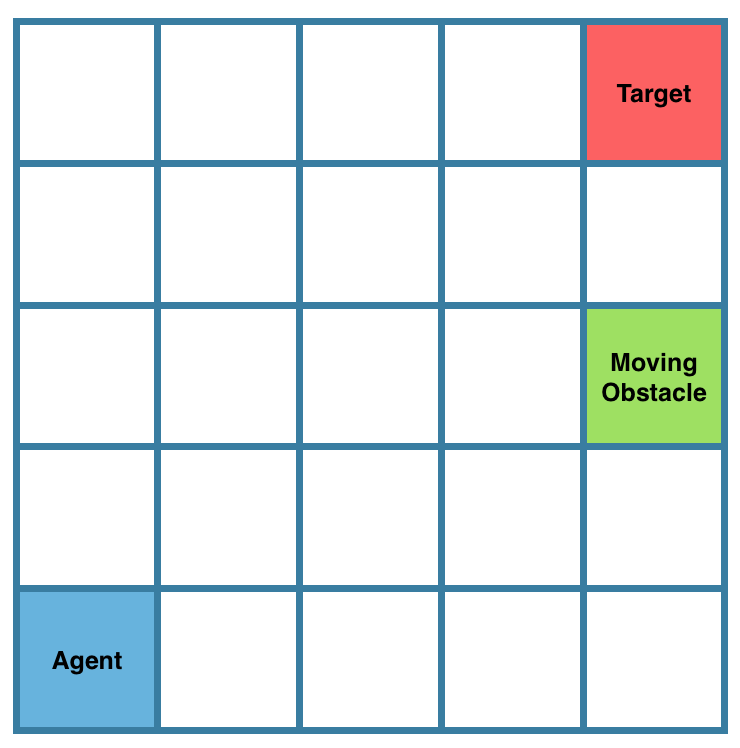
\includegraphics[width=0.15\textwidth]{images/gridworld.png}
%\vspace{-4mm}
  \caption{Simulated social navigation task.} \label{fig:gridworld}
\vspace{-7mm}
\end{figure}

% \begin{figure}[t]
%   \centering
%   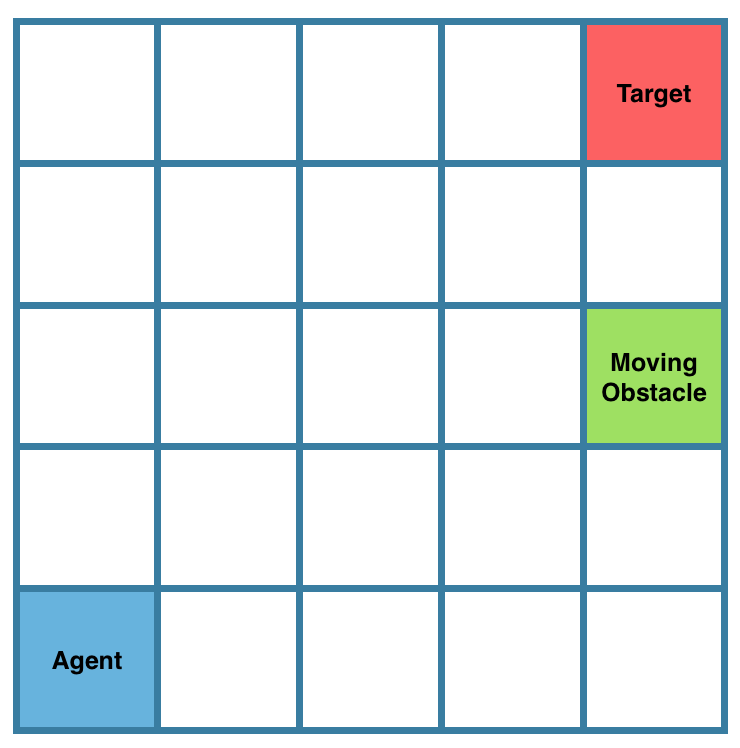
\includegraphics[bb=0 0 533 539,width=0.5\columnwidth]{images/gridworld.png}
%   \caption{Moving obstacle gridworld 	\label{fig:gridworld}}
% \end{figure}
We first manually define two ground truth reward functions, $R^{\mathcal{D}^*} = w^{\mathcal{D}^*}\phi(s,a)$, $R^{\mathcal{F}^*} = w^{\mathcal{F}^*}\phi(s,a)$, described further below. Then, we sample initial test states from a uniform distribution over the state space, over which we define $P^{s_1}_{test}$, for all experimental runs. These initial conditions, along with the optimal maximum-entropy policies for $R^{\mathcal{D}^*}$ and $R^{\mathcal{F}^*}$, allow us to compute feature expectations $\widetilde{\mu}^{\mathcal{D}_{test}}$ and $\widetilde{\mu}^{\mathcal{F}_{test}}$ respectively. For each experimental run, we then sample a set of initial training states, over which we define $P^{s_{1}}_{train}$, %\jm{this is another prior distribution, not a set of states}
and generate the respective feature expectations $\widetilde{\mu}^{\mathcal{D}_{train}}$, $\widetilde{\mu}^{\mathcal{F}_{train}}$. These feature expectations are used to learn reward functions and their corresponding  policies using each algorithm under evaluation. Each learned policy $\pi^*$ is then executed from initial states sampled from $P^{s_{1}}_{test}$ to determine $\mu^{\pi^*}|_{test}$, the feature expectations for the policy at those initial conditions. Finally, we compute the values of each policy, at those initial conditions, with respect to the two reward functions, $V^{\pi^*}_{\mathcal{D},test} = (w^{\mathcal{D}^*})^T\mu^{\pi^*}|_{test}$, $V^{\pi^*}_{\mathcal{F},test} = (w^{\mathcal{F}^*})^T\mu^{\pi^*}|_{test}$. A good algorithm will yield a high $V^{\pi^*}_{\mathcal{D},test}$ and a low $V^{\pi^*}_{\mathcal{F},test}$ .

\begin{figure*}[t]
   \hspace{-2mm}
  \begin{subfigure}[t]{0.57\columnwidth}
    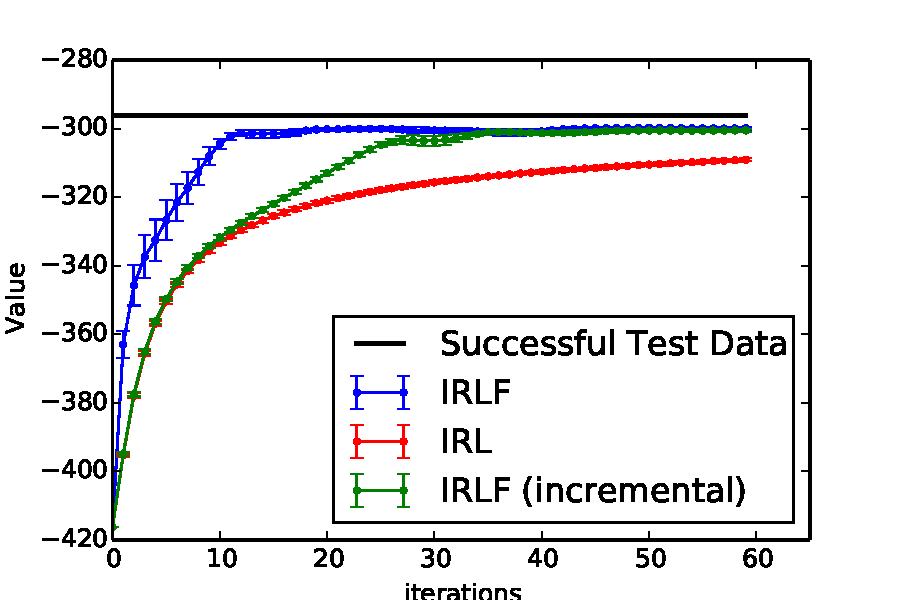
\includegraphics[clip=true,width=1.0\textwidth]{images/expert_apprentice_contrastive.pdf}
    \caption{Contrasting w.r.t.\ $w^{\mathcal{D}^*}$}
    \label{fig:toy_expert_apprentice_contrastive}
   \end{subfigure}
   \hspace{19mm}
   \begin{subfigure}[t]{0.57\columnwidth}
    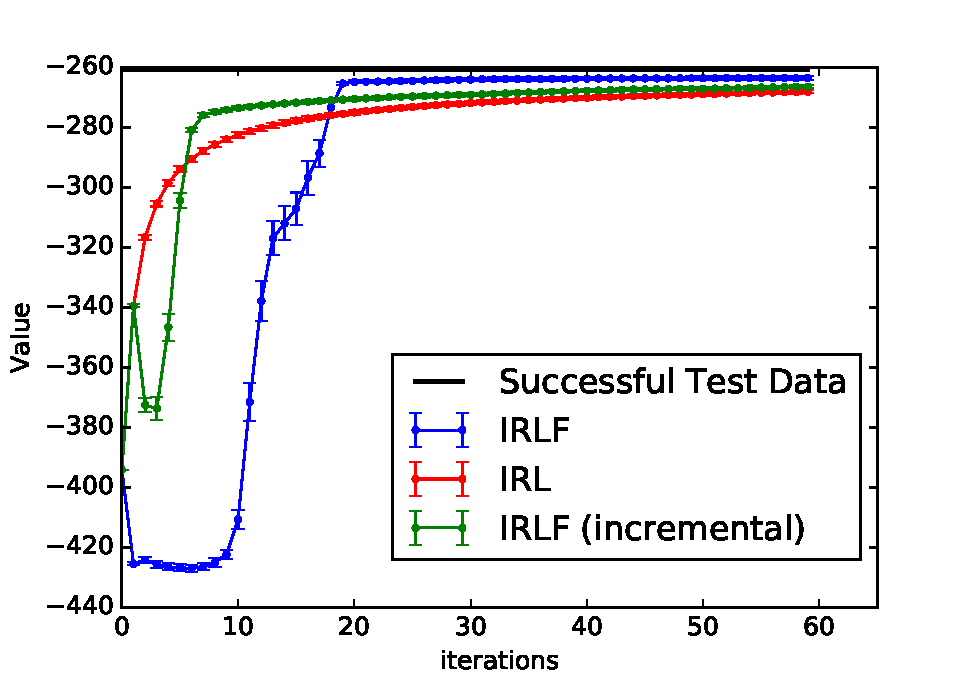
\includegraphics[trim=0.6cm 0.0cm 0.0cm 0.0cm,clip=true,width=0.93\textwidth]{images/over_expert_apprentice.pdf}
    \caption{Overlapping w.r.t.\ $w^{\mathcal{D}^*}$}
    \label{fig:toy_expert_apprentice_overlapping}
    \end{subfigure}
    \hspace{13mm}
    \begin{subfigure}[t]{0.57\columnwidth}
    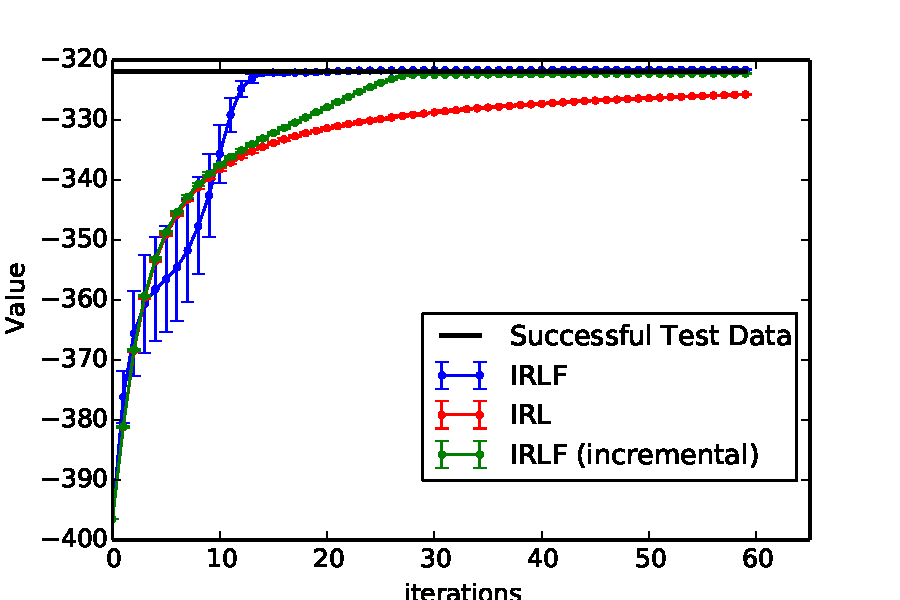
\includegraphics[trim=0.6cm 0.0cm 0.0cm 0.0cm,clip=true,width=0.95\textwidth]{images/expert_apprentice_complementary.pdf}
    \caption{Complementary w.r.t.\ $w^{\mathcal{D}^*}$}
    \label{fig:toy_expert_apprentice_complementary}
    \end{subfigure}
    \\

    \hspace{-2mm}
  \begin{subfigure}[t]{0.57\columnwidth}
    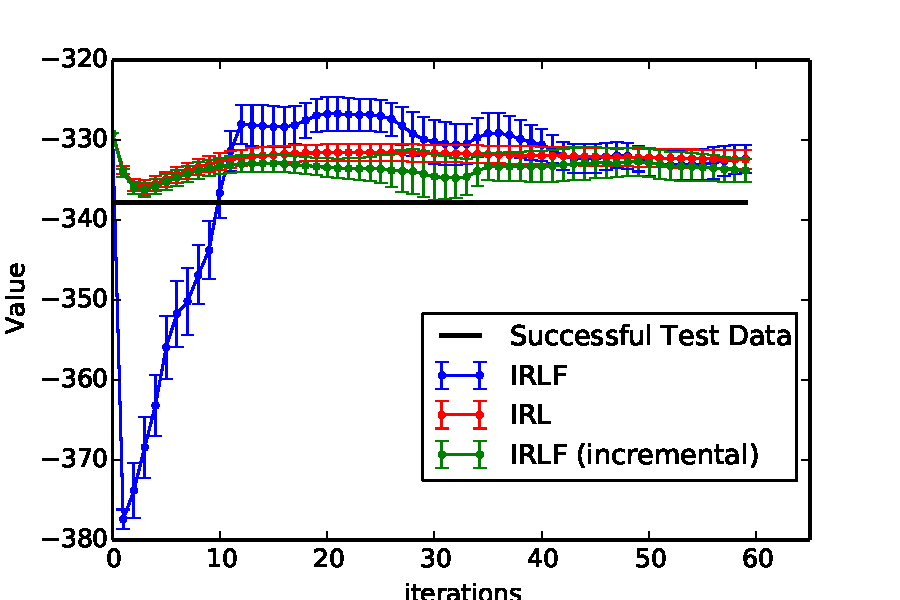
\includegraphics[clip=true,width=1.0\textwidth]{images/taboo_apprentice_contrastive.pdf}
    \caption{Contrasting w.r.t. $w^{\mathcal{F}^*}$}
    \label{fig:toy_taboo_apprentice_contrastive}
   \end{subfigure}
   \hspace{19mm}
   \begin{subfigure}[t]{0.57\columnwidth}
    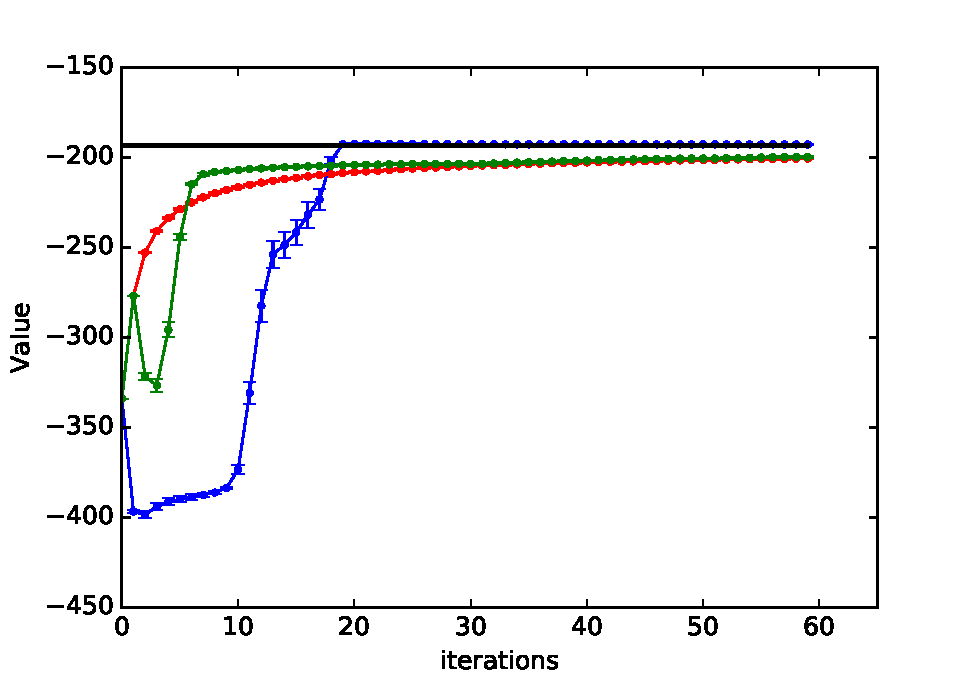
\includegraphics[trim=0.6cm 0.0cm 0.0cm 0.0cm,clip=true,width=0.93\textwidth]{images/over_taboo_apprentice.pdf}
    \caption{Overlapping w.r.t.\ $w^{\mathcal{F}^*}$}
    \label{fig:toy_taboo_apprentice_overlapping}
    \end{subfigure}
    \hspace{13mm}
    \begin{subfigure}[t]{0.57\columnwidth}
    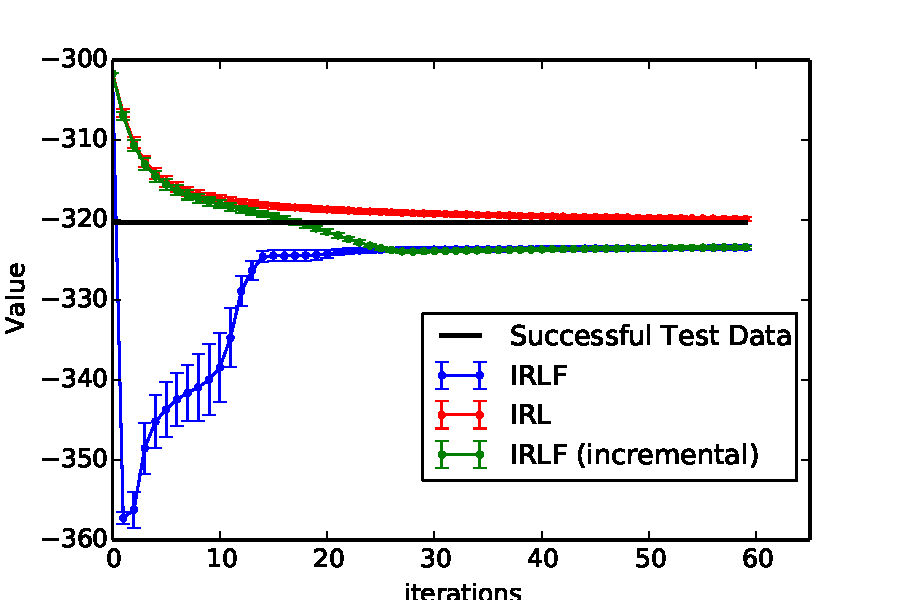
\includegraphics[trim=0.6cm 0.0cm 0.0cm 0.0cm,clip=true,width=0.95\textwidth]{images/taboo_apprentice_complementary.pdf}
     \caption{Complementary w.r.t.\ $w^{\mathcal{F}^*}$}
    \label{fig:toy_taboo_apprentice_complementary}
    \end{subfigure}
    % 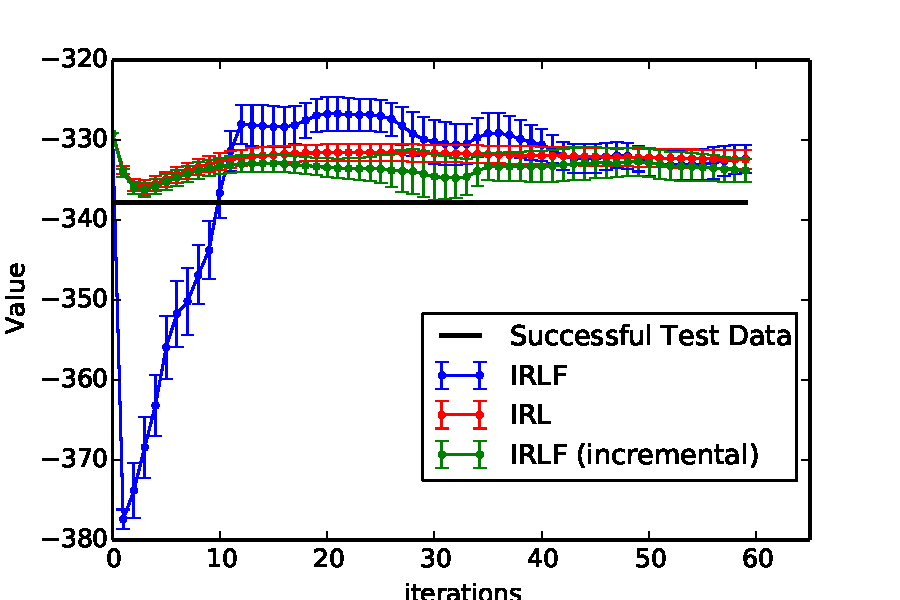
\includegraphics[clip=true,width=0.32\textwidth]{images/taboo_apprentice_contrastive.pdf}
    % 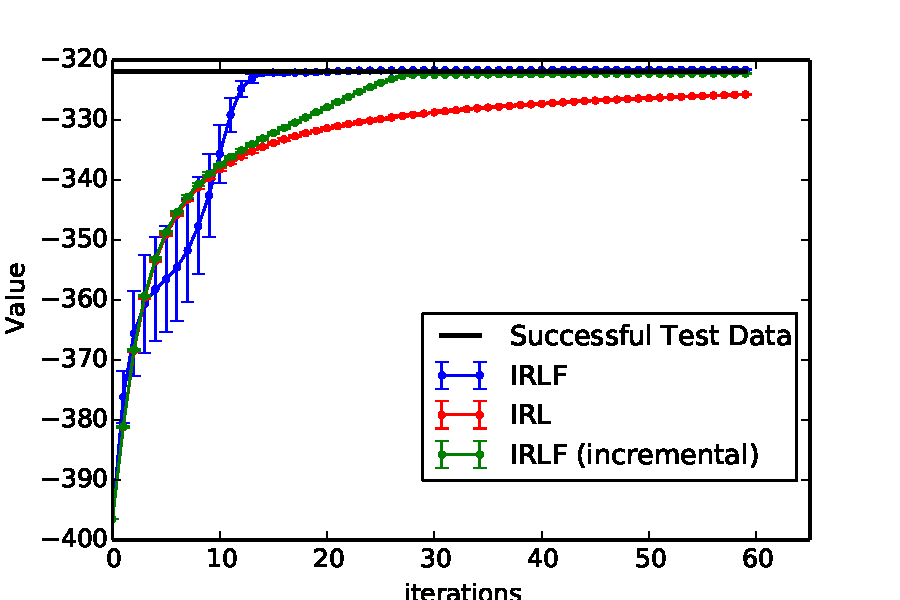
\includegraphics[clip=true,width=0.32\textwidth]{images/expert_apprentice_complementary.pdf}
    % 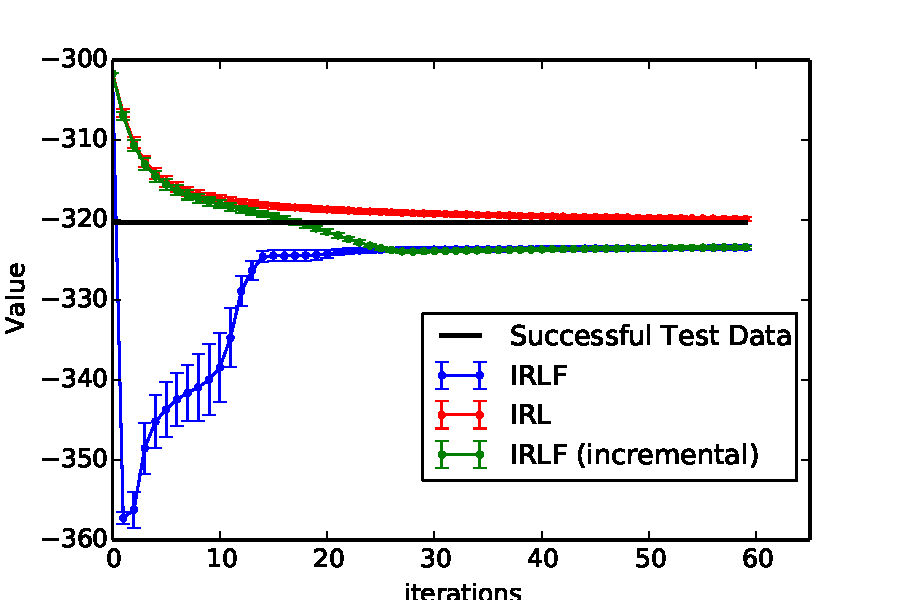
\includegraphics[clip=true,width=0.32\textwidth]{images/taboo_apprentice_complementary.pdf}
  \caption{Value over 60 iterations, for 20 runs in contrasting, complementary and overlapping simulated domains w.r.t. $w^{\mathcal{D}^*}$ and $w^{\mathcal{F}^*}$.}
  %\vspace{-3mm}
  \label{fig:complementary}

\end{figure*}

% The learner has access to two sets of trajectories, $\mathcal{D}_{train},\mathcal{F}_{train}$, of length $h = 15$. The trajectories in $\mathcal{D}_{train}$ are generated using a reward function $R^\mathcal{D} = w^\mathcal{D}\phi(s,a)$ and summarised by their feature expectations $\widetilde{\mu}^{\mathcal{D}_{train}}$. Likewise the tranjectories in $\mathcal{F}_{train}$ are generated by a reward function $R^\mathcal{F} = w^\mathcal{F}\phi(s,a)$ and summarised by $\widetilde{\mu}^{\mathcal{F}_{train}}$. The underlying ``true'' reward functions $R^\mathcal{D}$ and $R^\mathcal{F}$ represent, respectively, the positive aspects of the domains such as reaching the target, and its negative aspects such as hitting the obstacle. The reward functions are not known to the learner. \jm{need more detail on the reward function. What are the specific numbers for these things? Otherwise, we need to make the code available and link it, for this to be reproducible.}

% Two more sets of trajectories, namely $\mathcal{D}_{test}$ and $ \mathcal{F}_{test}$, are used to assess the learner's performance on the task. The evaluation takes place by measuring the value accumulated by the agent based on the respective dataset's true reward function. Using equation \eqref{eq:parametrized_value} this is simply,
% \begin{align}
% &V^{\pi}_{\mathcal{D}} = (w^\mathcal{D})^T\mu^\pi|_\mathcal{D}\\
% &V^{\pi}_{\mathcal{F}} = (w^\mathcal{F})^T\mu^\pi|_\mathcal{F}. \label{eq:value_on_expert}
% \end{align}
% In other words, we can use the weights for each of the reward functions, along with the feature expectations associated with the execution of a policy from a certain set of initial conditions, to measure the performance of the agent with respect to that reward function. If therefore follows that a well-performing algorithm will maximise $V^{\pi}_{\mathcal{D}_{test}}$ and minimise $V^{\pi}_{\mathcal{F}_{test}}$. 

% In our experiments we fix $10$ test states (and their respective feature expectations) and perform experimental runs, for which we train our IRLF algorithm and its original counterpart, the MaxCausEnt IRL algorithm, on randomised initial conditions. The performance of the learned reward functions (and policies) at the fixed initial test states is evaluated using \eqref{eq:value_on_expert}. \jm{this sentence doesnt make sense.}\ks{I wanted to say that we learn on some initial conditons and test on others.}

Within this domain, we consider three scenarios that differ in how $R^{\mathcal{D}^*}$ and $R^{\mathcal{F}^*}$ are defined.  In the \emph{contrasting scenario}, $w^{\mathcal{D}^*}$ rewards reaching the target and avoiding the obstacle, while $w^{\mathcal{F}^*}$ rewards being in the same cell as the obstacle.  This scenario examines the value of completely failed demonstrations when the successful demonstrations already show the complete desired behaviour. 

In the \emph{overlapping scenario}, $w^{\mathcal{D}^*}$ is as before but $w^{\mathcal{F}^*}$ rewards not only colliding with the obstacle, but also reaching the target. This scenario examines the value of failed demonstrations when they are similar in some respects to the successful demonstrations. 

In the \emph{complementary scenario}, $w^{\mathcal{D}^*}$ rewards only reaching the target, while $w^{\mathcal{F}^*}$ only rewards hitting the obstacle. This scenario examines the value of failed demonstrations when the successful demonstrations do not fully disambiguate the desired behaviour.

Figures \ref{fig:toy_expert_apprentice_contrastive} and \ref{fig:toy_taboo_apprentice_contrastive} compare the performance of IRLF, with and without incremental updates to $\lambda$, to that of IRL in the contrasting scenario. Both versions of IRLF successfully utilise failed demonstrations to learn better and faster than IRL in terms of $V^{\pi^*}_{\mathcal{D},test}$.  They achieve similar performance to IRL in terms of $V^{\pi^*}_{\mathcal{F},test}$.  

Figures \ref{fig:toy_expert_apprentice_overlapping} and \ref{fig:toy_taboo_apprentice_overlapping} show results for the overlapping scenario. Even in this challenging setting, IRLF learns better than IRL, demonstrating the resilience of our method to the fact that some successful and failed trajectories might be similar and showing that our method can exploit the additional data found in failed trajectories without negative side effects. 

Finally, Figures \ref{fig:toy_expert_apprentice_complementary} and \ref{fig:toy_taboo_apprentice_complementary} show similar results for the complementary scenario.  The IRLF methods again perform better in terms of $V^{\pi^*}_{\mathcal{D},test}$ but now also perform better in terms of $V^{\pi^*}_{\mathcal{F},test}$.  In fact, they outperform even the successful data in terms of $V^{\pi^*}_{\mathcal{F},test}$, a consequence of the complementary nature of the reward functions. 

IRLF's performance with respect to $V^{\pi^*}_{\mathcal{F},test}$ (Figure \ref{fig:complementary} bottom row) illustrates how the algorithm gives priority to successful demonstrations when necessary. For the contrasting scenario, the probability of approaching the obstacle is already low for $w^{\mathcal{D}^*}$; therefore, IRL and IRLF behave similarly with respect to $w^{\mathcal{F}^*}$. In the ovelapping scenario, IRLF gives priority to reaching the target quickly, since this matches the behavior in the successful demonstrations (even though it is discouraged from doing so by the failed demonstrations). Doing so means accumulating more value in terms of $V^{\pi^*}_{\mathcal{F},test}$. In the complementary scenario, since it is possible to satisfy both objectives simultaneously (reaching the target and avoiding obstacles), IRLF finds a reward function that performs well with respect to the succesful demonstrations while at the same time having a lower value with respect to the failed demonstrations.

 In all scenarios, IRLF is more stable with incremental updates than without.  In the contrasting and complementary scenarios, IRLF with incremental updates learns more slowly, while in the overlapping scenario it learns faster initially but plateaus slightly lower.

 In the experiments above, all methods received successful and failed demonstrations from five initial states. Hence, the results do not address how the number of succesful demonstrations given to the two learners affects their performance on the test set. In the complementary scenario, failed demonstrations are obviously important regardless of how many succesful demonstrations are available. In the other scenarios, however, it is not clear whether failed demonstrations are still useful even when successful demonstrations are abundant.

To test this, we repeated our experiments in the constrasting scenario but with 5, 50, 200 and 2000 initial states for successful demonstrations, while keeping the failed demonstrations to 5. For each algorithm, we plot  $(w^{\mathcal{D}^*})^T\widetilde{\mu}^{\mathcal{D}_{test}}$ - $V^{\pi^*}_{\mathcal{D},test}$ after 60 iterations of the algorithm. The smaller this value, the closer the learner comes to replicating the expert on the test set of initial states. The results, shown in Figure \ref{fig:data_size}, demonstrate that IRLF maintains its superiority over IRL even if the number of initial states for which demonstrations are given rises significantly. 

\begin{figure}
	\vspace{-2mm}
	\centering
 	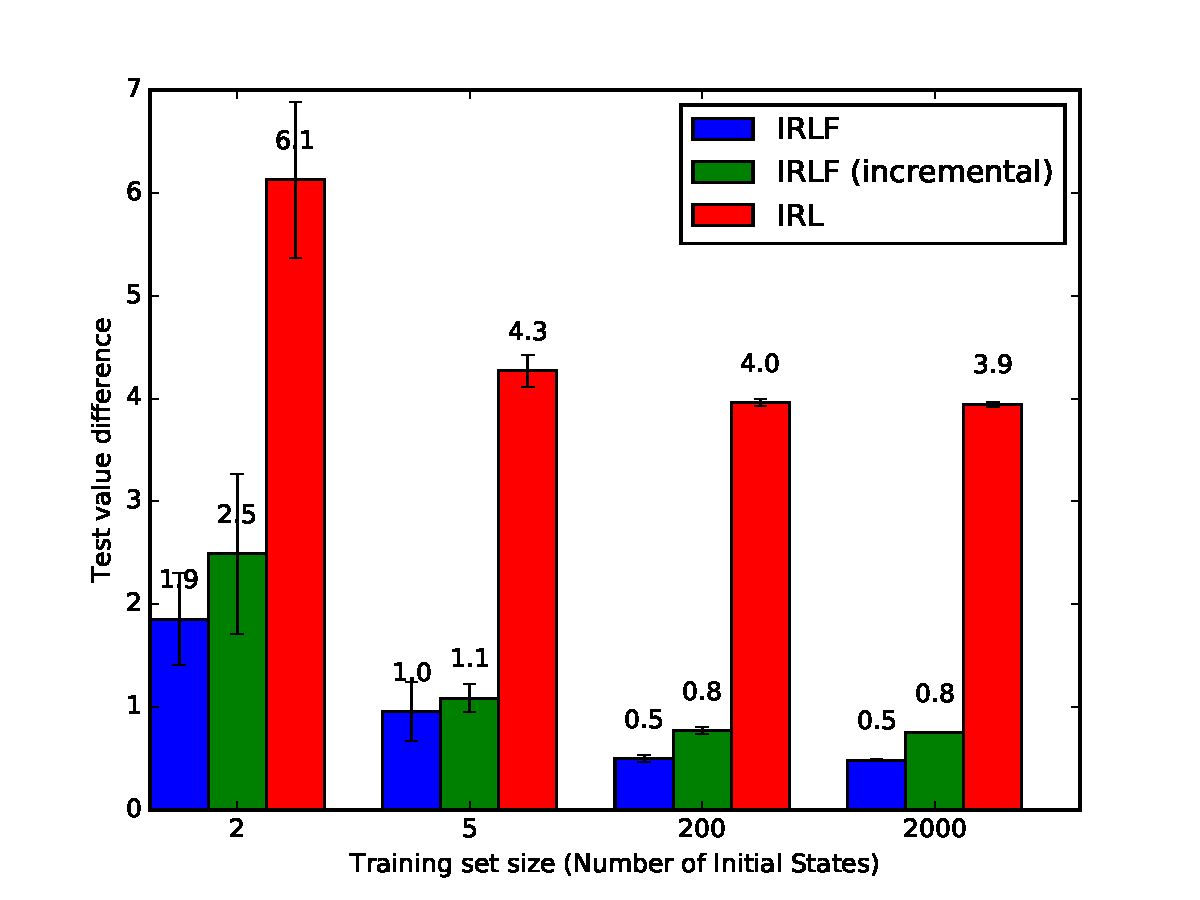
\includegraphics[clip=true,width=0.35\textwidth]{images/data_size.pdf}
 	\caption{Performance of all three methods in the constrasting scenario for different numbers of initial states.}
 	\label{fig:data_size}
 	\vspace{-2mm}
\end{figure}

To shed more light on IRLF's behaviour, Figure \ref{fig:rf_plot} plots the original and learned reward functions for IRL and IRLF for the contrasting scenario. In the original reward function $w^{\mathcal{D}^*}$ (Figure \ref{fig:rf_plot_good}), the obstacle is in cell [2,2] and the goal in cell [4,4], which explains the dips and spikes in those locations.  The reward function learned by IRL (Figure \ref{fig:rf_plot_irl}) is flat in the area of the obstacle. However, IRLF, by employing $w^{\mathcal{F}^*}$ (Figure \ref{fig:rf_plot_bad}) learns a reward function (\ref{fig:rf_plot_irlf}) that properly assigns a low reward to the obstacle and its surroundings. The reward function resulting from IRLF can therefore generalise better to unseen initial conditions and environments.


\begin{figure*}[thb]
  \centering
  \begin{subfigure}[b]{0.45\columnwidth}
  	\hspace{-6mm}
    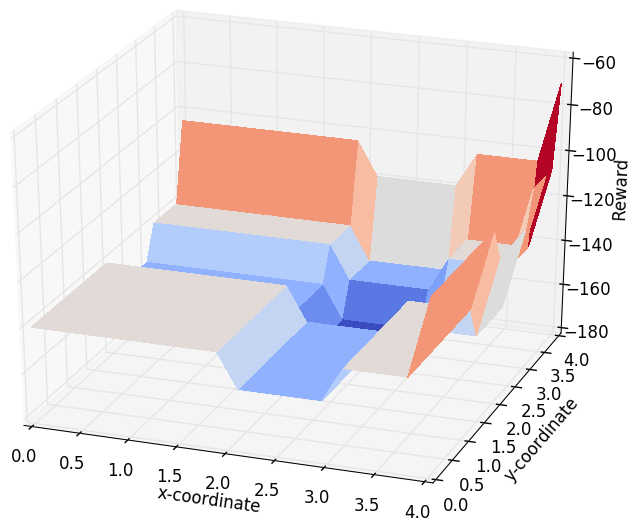
\includegraphics[clip=true,width=\textwidth]{images/RF_D.png}

    
    \caption{\ $w^{\mathcal{D}^*}$}
    \label{fig:rf_plot_good}
  \end{subfigure}
  %\hfill
  \begin{subfigure}[b]{0.45\columnwidth}
  \hspace{-3mm}
    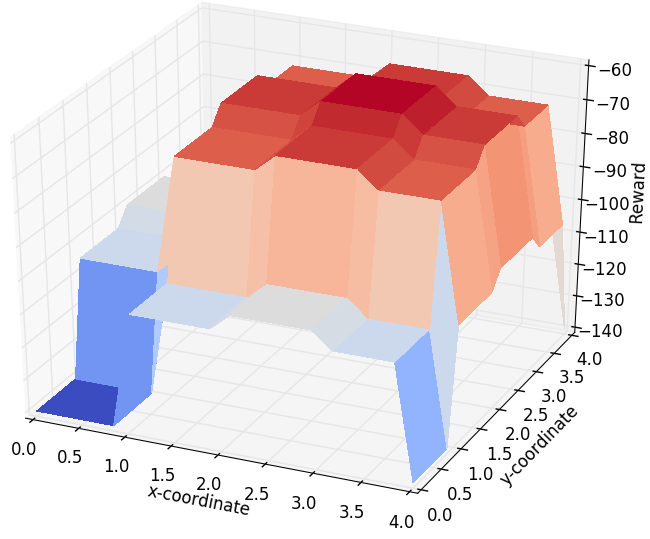
\includegraphics[clip=true,width=\textwidth]{images/RF_F.png}

    
    \caption{\ $w^{\mathcal{F}^*}$}
    \label{fig:rf_plot_bad}
  \end{subfigure}  
  \label{fig:contrastive}
  \begin{subfigure}[b]{0.45\columnwidth}

    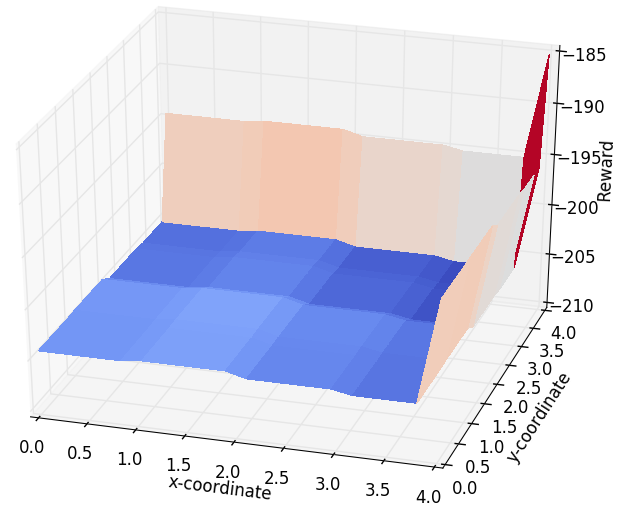
\includegraphics[clip=true,width=\textwidth]{images/RF_IRL.png}
    \caption{IRL}
    \label{fig:rf_plot_irl}
  \end{subfigure}
  %\hfill
  \begin{subfigure}[b]{0.45\columnwidth}
  	\hspace{5mm}
    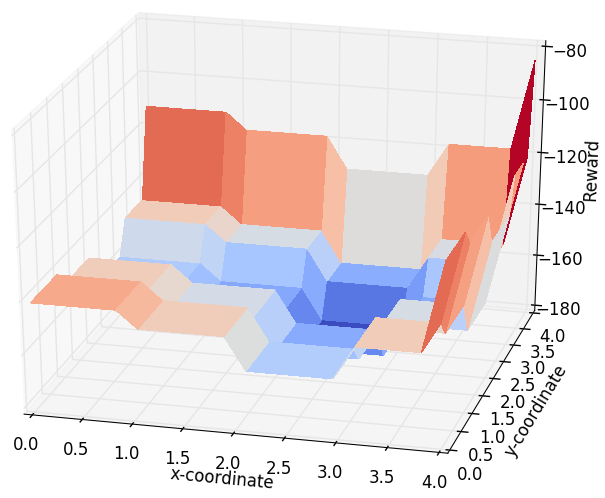
\includegraphics[clip=true,width=\textwidth]{images/RF_IRLF.png}
    \caption{IRLF}
    \label{fig:rf_plot_irlf}
  \end{subfigure}  
  %\vspace{-3mm}
  \caption{The original reward and learned reward functions for the two algorithms. Obstacle is static at [2,2]\ }
  %\vspace{-3mm}
  \label{fig:rf_plot}
\end{figure*}


% \begin{table}[]
% \centering

% \label{tab:results}
% \begin{tabular}{|l|l|l|l|}
% \hline
%            & $\theta_e(\Phi_{a}-\Phi_{e)}$& $\theta_t(\Phi_{a}-\Phi_{t)}$ & $|\pi_a - \pi_t|$ (\%) \\ \hline
% Original   & -6.125(2.06)        & 2.41(1.82)         & 15                    \\ \hline
% Our Method & 0(0.2)              & 0.02(0.167)        & 10                    \\ \hline
% \end{tabular}
% \caption{Results on test set after 20 runs of random initial conditions. $\theta_e$ represent reward weights, $\pi$ represents policy and $\Phi$ represents feature expectations. The subscripts $a,e,t$ represent the apprentice, expert and taboo agents respectively. \jm{This table needs to be cleaned up. Try to keep the same number of significant figures in all entries.}}
% \end{table}
% REAL DATA SECTION %

\subsection{Simulated Factory Domain}
Our second simulated domain is the \emph{Factory} benchmark problem proposed by Dearden \& Boutilier \cite{dearden1997abstraction}. In this domain, an autonomous agent is tasked with building an object according to specifications, which involves some sequence of shaping, painting, cleaning and assembly operations on its parts. Each individual operation costs some time and may have a probabilistic outcome, possibly resulting in unwanted side effects on the condition of each of the parts. Furthermore, there are precedence conditions on some of these operations -- for instance, parts must be shaped before they can be assembled. The goal of this domain is to produce the object in the most cost-efficient way.

While this problem has been previously tackled from the perspective of off-line decision-theoretic planning, it is a suitable domain to demonstrate the applicability of learning from demonstration, and in particular of IRLF. In a real manufacturing problem, human demonstrations on how to properly execute the manufacturing task, as well as failed demonstrations, in which the resulting object did not meet the quality specifications, would be readily available. Furthermore, consider a situation where the conditions in the factory problem may be subject to changes (for example, in the shapes or sizes of the parts) which may affect the optimal manufacturing policy. Learning a reward function, as opposed to learning a policy from demonstration, would make it easier for an autonomous agent to adapt to these changes.

\begin{figure}[tbh]
	\centering
%	\hspace{-5cm}
      \begin{subfigure}[b]{0.45\columnwidth}
      \hspace{-11mm}
    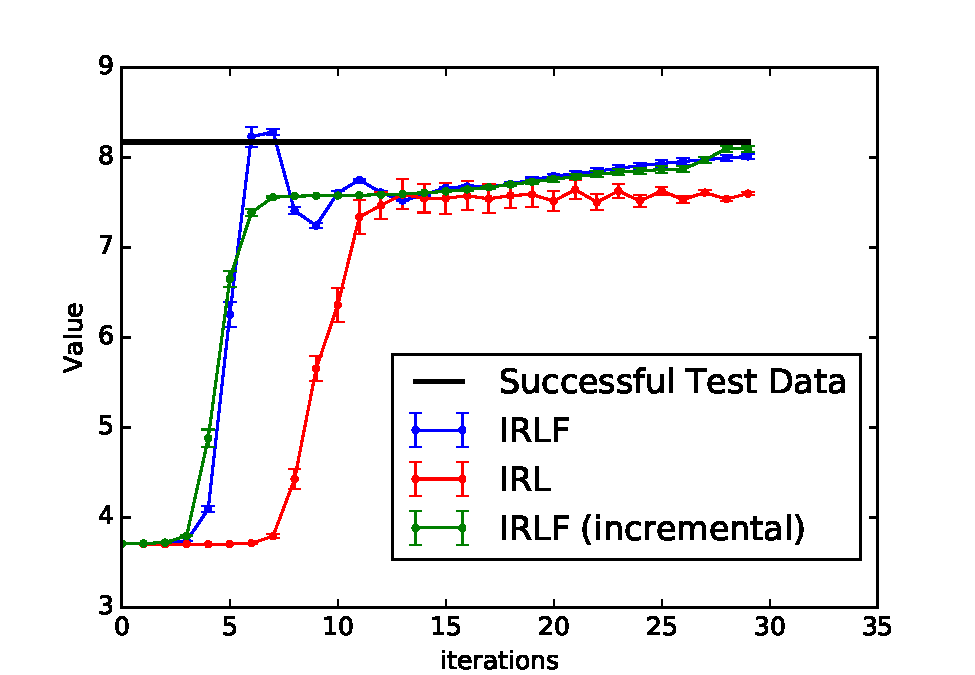
\includegraphics[clip=true,width=1.25\textwidth]{images/factory_1.pdf}
    \caption{Value w.r.t.\ $w^{\mathcal{D}^*}$}
    \label{fig:factory_1}
  \end{subfigure}
 % \hspace{5mm}
  \begin{subfigure}[b]{0.45\columnwidth}
    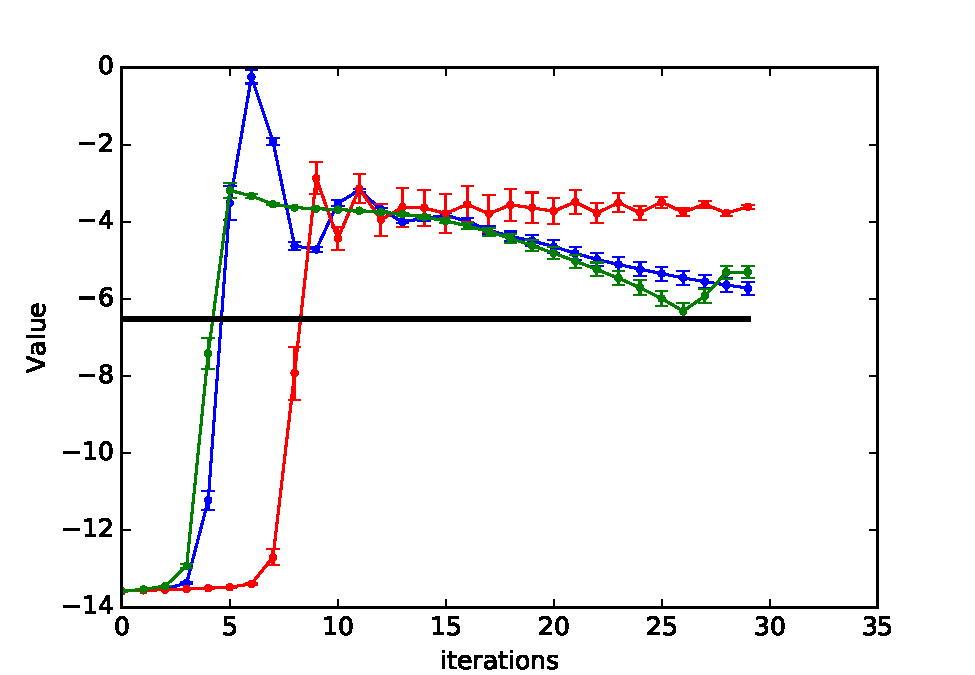
\includegraphics[trim=0.8cm 0.0cm 0.0cm 0.0cm,clip=true,width=1.20\textwidth]{images/factory_2.pdf}
    \caption{Value w.r.t.\ $w^{\mathcal{F}^*}$}
    \label{fig:factory_2}
  \end{subfigure} 

  %\vspace{-3mm}
  \caption{Value over 30 iterations, for 15 runs of learning in the Factory domain.}
  %\vspace{-3mm}
  \label{fig:factory_results}

\end{figure}

Our instantiation of the Factory problem follows Dearden \& Boutilier's description \cite{dearden1997abstraction} (\emph{c.f.} Section A.2). It has $512$ states, factored into $9$ binary variables, and $10$ actions. The expert demonstrations were drawn from the optimal policy for that domain according to its original additive rewards ($w^{\mathcal{D}^*}_i$, Table \ref{tab:factory_reward}), while the failed demonstrations were drawn from a policy derived from a different reward function ($w^{\mathcal{F}^*}_i$, Table \ref{tab:factory_reward}). Note that we consider only $5$ features, corresponding to those state factors that have non-zero rewards. Each demonstration starts from random initial conditions and the evaluation proceeds in an identical manner to Section \ref{sec:sim_nav}.

\begin{table}[]
\centering

\begin{tabular}{|c|c|c|c|}
\hline
\begin{tabular}[c]{@{}c@{}}Feature\\Index $i$\end{tabular} & Proposition & $w^{\mathcal{D}^*}_i$ & $w^{\mathcal{F}^*}_i$\\ \hline
1                                                         & AClean      & 0.1 & 1    \\ \hline
2                                                         & BClean      & 0.1 & -0.1    \\ \hline
3                                                         & APainted    & 0.2 & 0.4    \\ \hline
4                                                         & BPainted    & 0.2 & 0    \\ \hline
5                                                         & Joined      & 0.4 & -2    \\ \hline
\end{tabular}
\caption{Reward functions for the Factory domain.\label{tab:factory_reward}}
\end{table}

% \begin{figure}[htb]     
%   \centering
%     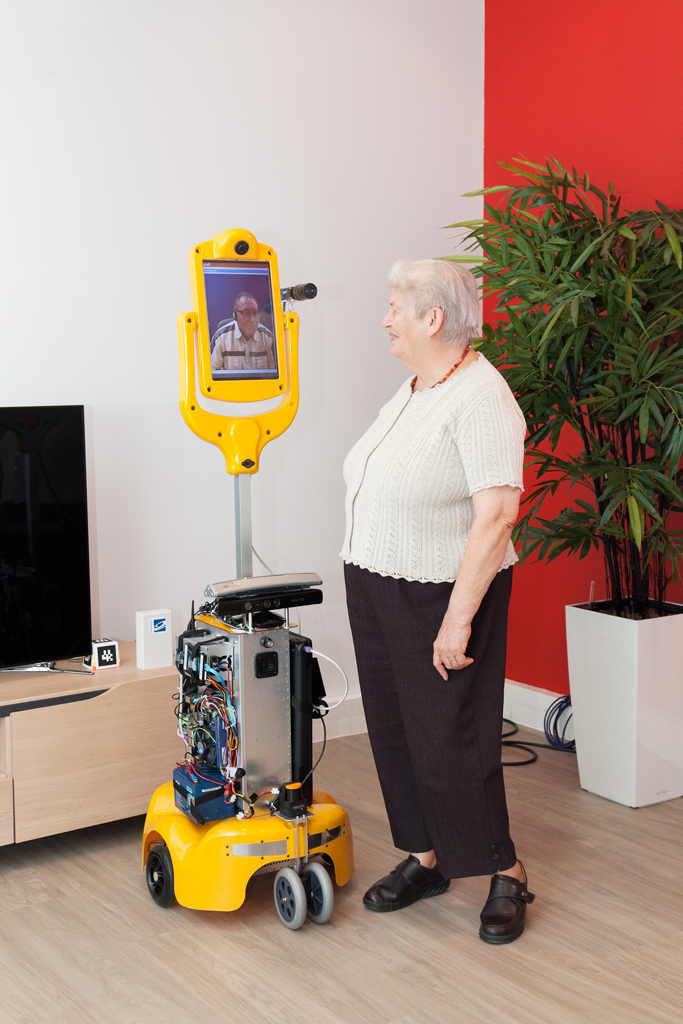
\includegraphics[width=0.75\columnwidth]{images/robot.jpg}
%   \caption{The semi-autonomous telepresence robot used in our experiments.}
%   \label{fig:teresa_subject}
% \end{figure}

Figure \ref{fig:factory_results} shows the results, which are consistent with our previous observations. Figure \ref{fig:factory_1} shows that the reward function learned using IRLF is capable of yielding a policy that achieves a higher $V^{\pi^*}_{\mathcal{D},test}$ than IRL, and very close to that of the original policy. Furthermore, Figure \ref{fig:factory_2} shows that IRLF is capable of achieving lower $V^{\pi^*}_{\mathcal{F},test}$ than IRL. These results not only demonstrate the stability and reliability of IRLF, but further confirm the usefulness of failed demonstrations in inverse reinforcement learning.



\subsection{Real Navigation Domain}

We also evaluate the performance of IRLF on a social navigation dataset gathered using a real robot. The robot, shown in Figure \ref{fig:teresa_subject}, is a commercially available telepresence system that has been augmented with extra sensors and processors. The collected dataset consists of 47 trajectories of an expert navigating the robot towards an interaction target while avoiding a moving or standing  person in a socially appropriate way. The positions of the people and the robot were accurately recorded using a motion capture system covering an area of $5m \times 5m$. A sample of the collected trajectories are shown in Figure \ref{fig:data}. 

For safety reasons, the failed dataset $\mathcal{F}$, which consists of $59$ trajectories, was collected by driving the robot in a simulator in a way that intentionally violates social norms, e.g., running into, following, or standing next to people. 

%\vspace{1mm}
\begin{figure}[t]     
%  \vspace{-2mm}
  \centering
    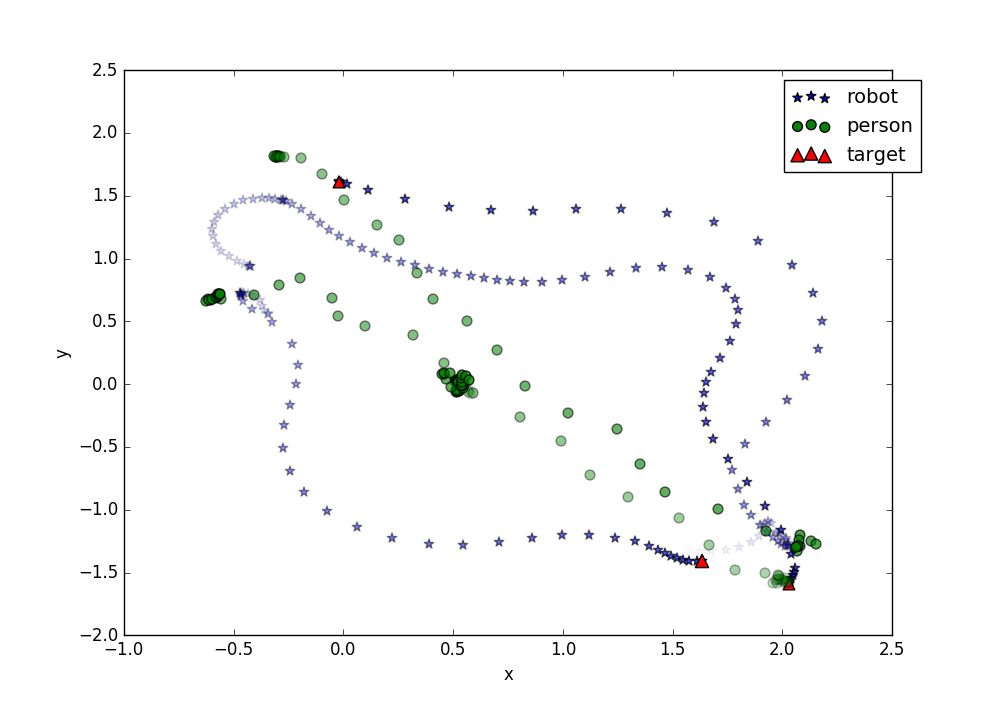
\includegraphics[width=0.6\columnwidth]{images/data_plot.png}
  \caption{A sample of trajectories from the real navigation domain data set. Darker dots occur later in time.}
  \label{fig:data}
\end{figure}

To model this domain as an MDP, we define a state space $S$ consisting of discretised positions for both the obstacle and the robot, as well as the discretised orientation of the obstacle, yielding a total of $837,808$ states. The action space consists of eight possible directions for robot movement, and an action that stops the robot. Using $\mathcal{D}$, we learned a factored stochastic transition function $T$. Furthermore, we defined a feature set $\phi(s,a)$ of $1401$ binary features, encoding the relative position of the robot from both the target and the obstacle, as well as their relative orientations. 

Applying IRL and IRLF to this domain is straightforward.  However, measuring performance is not, because we do not have access to the ground truth reward function needed to compute a policy's value. In previous work on IRL, researchers have taken multiple approaches to evaluation.  Some have considered simulated domains \cite{levine2011nonlinear,syed2007game,rothkopf2011preference} as in our results above, where a ground truth reward function is available. Others have considered real-world data but relied on qualitative evaluation \cite{ratliff2006maximum}, domain-specific performance measures \cite{neu2009training} or ad-hoc performance measures \cite{vasquez2014inverse}.

Since none of these approaches is entirely satisfactory, we adopt a different approach. First, we apply IRL to both $\mathcal{D}$ and $\mathcal{F}$ and derive reward functions, $R^{\mathcal{D}}$ and $R^{\mathcal{F}}$ and their respective weights $w^{\mathcal{D}^*}$ and $w^{\mathcal{F}^*}$, which we thereafter treat as ground truth.
Because MDPs are generative models, we can use these two separate reward functions to generate data while preserving access to the ground-truth reward functions that are so essential to evaluation. We are therefore able to conduct an evaluation analogous to the done in the simulated navigation domain, with the key difference that the $w^{\mathcal{D}^*}$ and $w^{\mathcal{F}^*}$ are learned from real data. 

Figure \ref{fig:paths}, which shows example trajectories generated by these reward functions, confirms that $w^{\mathcal{D}^*}$ produces human-like trajectories, while $w^{\mathcal{F}^*}$ generates inappropriate beha\-viour. These two reward functions can therefore be considered to be two separate agents whose demonstrations IRLF uses in order to learn a single reward function in a principled manner.

Figure \ref{fig:real_data} shows the results of our experiments on the real data, averaged across 6 independent runs. These results de\-monstrate that both versions of IRLF substantially outperform IRL with respect to $w^{\mathcal{D}^*}$.  The performance of all methods is similar with respect to $w^{\mathcal{F}^*}$, which suggests that, in this domain, imitating good behaviour is sufficient to score very low with respect to $w^{\mathcal{F}^*}$.  IRLF without incremental updates to $\lambda$ clearly oscillates, as expected, but still converges, while IRLF with incremental updates is stable and achieves a higher value than IRL.
%
Overall, the consistency of these results with those of the simulated domain provides further confirmation that failed demonstrations are useful for IRL, allowing it to generalise better to new initial conditions.  Furthermore, IRLF is a useful method for exploiting this data.

\begin{figure}[htb]
\vspace{-2mm}
%  hspace{-16pt}
	\centering
	\hspace{-6mm}
    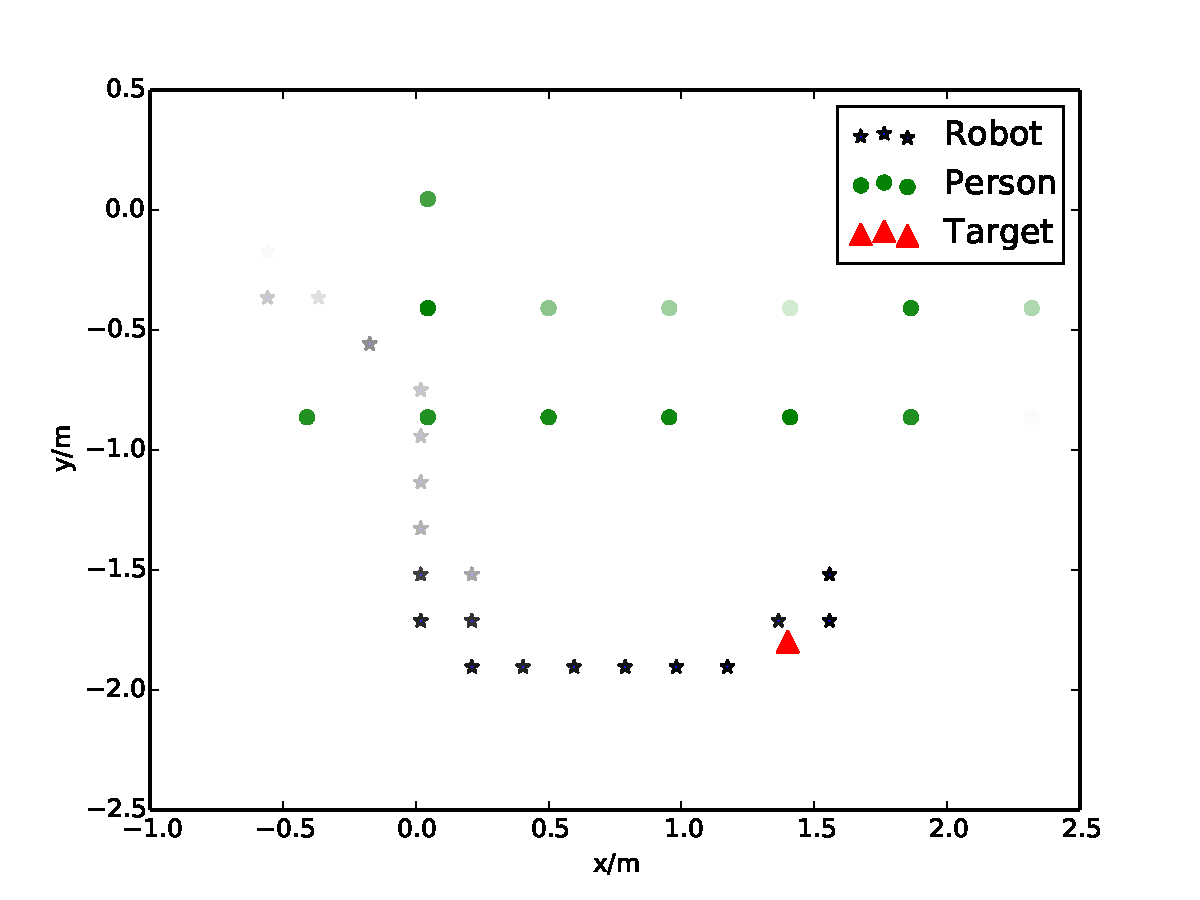
\includegraphics[scale = 0.22]{images/gp.pdf}
    \hspace{-2mm}
    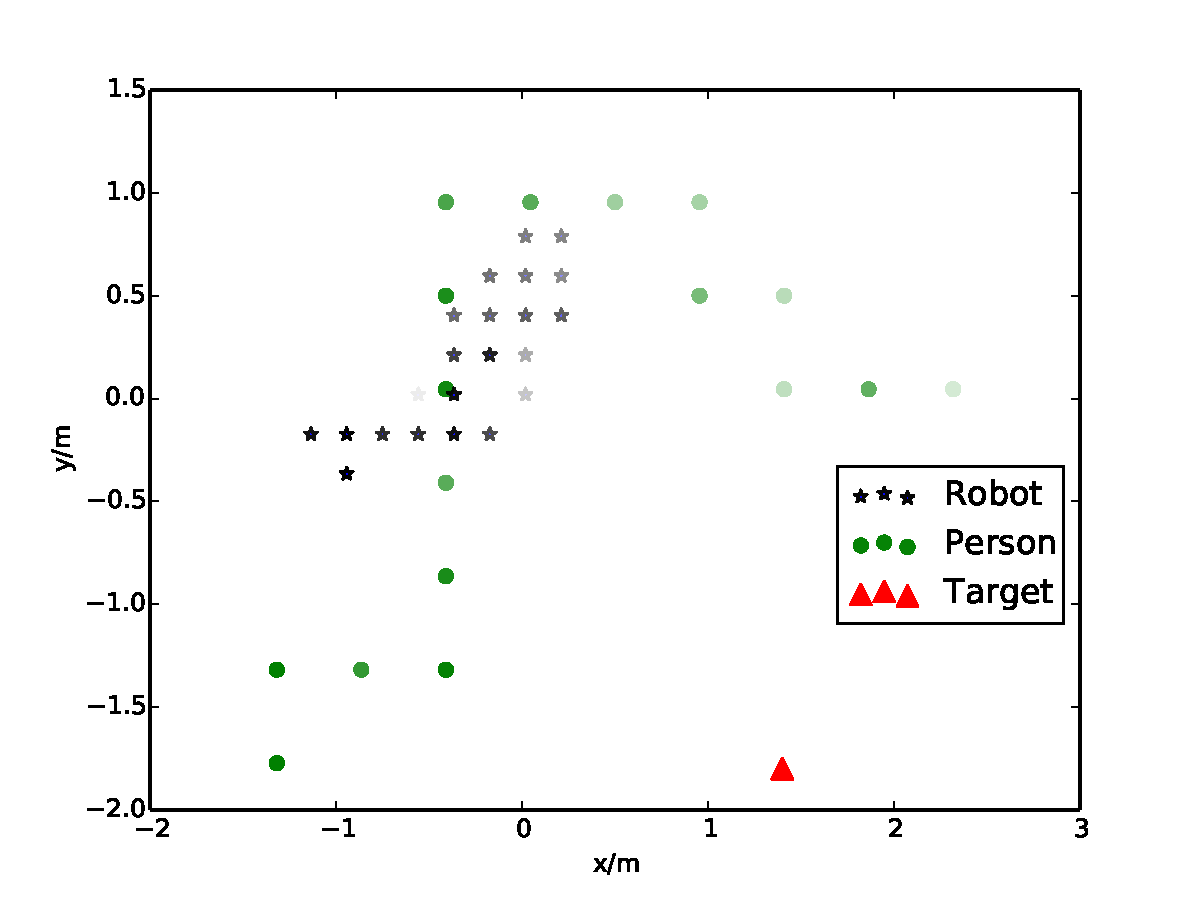
\includegraphics[scale = 0.22]{images/bp.pdf}
  \caption{Sample trajectories from $w^{\mathcal{D}^*}$ (top) and $w^{\mathcal{F}^*}$ (bottom). Darker dots occur later in time.} %These reward functions were learned from real data. The alpha channel denotes time}}
  \label{fig:paths}
%\vspace{-2mm}
\end{figure}

\begin{figure}[h!]
	\vspace{-2mm}
	\centering
	\hspace{-5mm}
    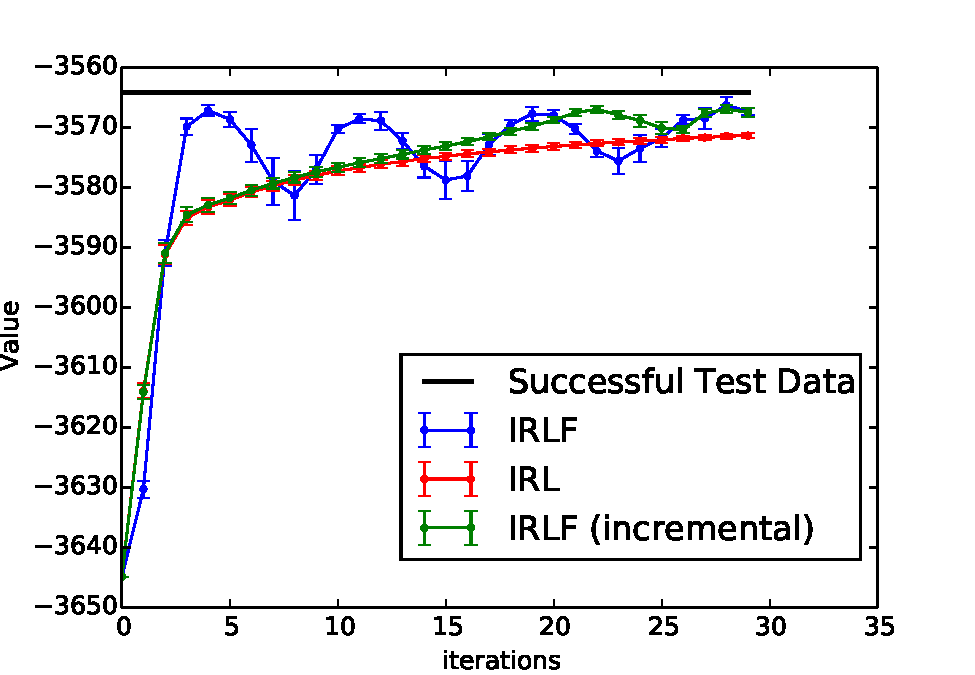
\includegraphics[trim=0.5cm 0.5cm 0.2cm 0.2,clip=true,width=0.24\textwidth]{images/expert_apprentice_real.pdf}
    %\hspace{mm}
    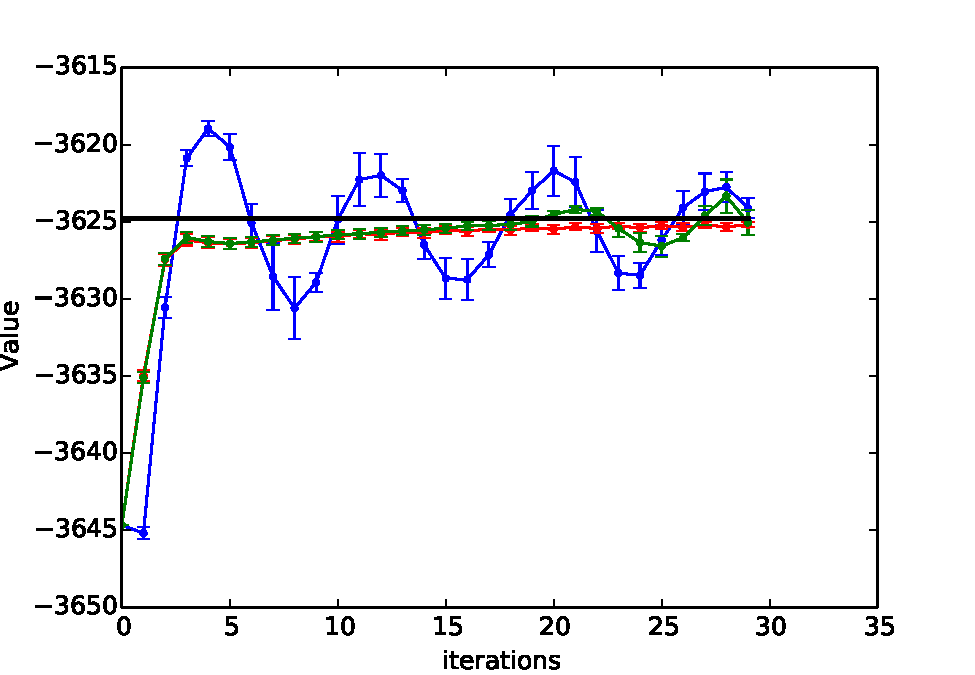
\includegraphics[trim=0.5cm 0.5cm 0.2cm 0.2,clip=true,width=0.24\textwidth]{images/taboo_apprentice_real.pdf}
  \caption{Value over 30 iterations, for 6 runs on real data w.r.t.\ $w^{\mathcal{D}^*}$ (top) and $w^{\mathcal{F}^*}$(bottom).}
  %\vspace{-4mm}
  \label{fig:real_data}
\end{figure}
%\vspace{-2mm}

%\vspace{-2mm}
\section{Conclusions and Future Work}

% \sw{This can be modeled on the new abstract once it's written.  We do need some future work ideas.} \jm{Perhaps we can mention further robot tests and validation of these results as future work. There was also this idea on the table of coupling this learning from failure approach with other IRL / LfD algorithms}

This paper introduced IRLF, the first inverse reinforcement learning algorithm that can learn from successful as well as failed demonstrations simultaneously. Starting from the maximum causal entropy IRL method, we proposed a new constrained optimisation formulation that accommodates both types of demonstrations while remaining convex and derived update rules for learning reward functions and policies. Our simulated navigation experiments investigated the properties of IRLF in cases where the succesful and failed demonstrations are either constrasting, overlapping, or complementary. The results in the overlapping scenario show that IRLF works even if the failed demonstrations are similar to the successful ones. We also presented results on a simulated factory domain as well as on real robot data from a social navigation task. These results clearly suggest that IRLF consistently learns faster and generalises better than the original IRL algorithm in consideration. In future work, we aim to investigate whether other IRL methods can also be extended to exploit failed demonstrations. In addition, we plan to conduct more experiments with real robots, including deploying an IRLF-learned policy on a robot.

%  A clear direction for further reasearch is to investigate wether other IRL algorithms can be extended in a similar way. Furthermore, the emerging evidence of the benefits of learning to avoid certain solutions, suggests that the idea can be applied to related fields such as structured prediction.


% In this paper we have introduced a new framework for Inverse Reinforcement Learning that allows an agent to not only imitate certain behaviours but to also avoid others. The benefits this approach is that it allows otherwise useless data to be used and further enables a designer to inject prior information in the learning, by specifying, through simulated data, what behaviours should be avoided. We have derived a theoretically sound method by directly modifying the derivation of the Maximum Entropy and carrying that through to MaxEnt IRL, providing solutions to the computational obstacles that arise. We have further performed exhaustive experiments in a toy domain, that clearly demonstrate that our method can generalise much better that the baseline IRL algorithm. Finally we have performed learning on real data, again showing that our method is superior to the baseline.  
\vspace{-2mm}
\section{Acknowledgements}
This work is funded by the EC-FP7 under grant agreement no.\ 611153 (TERESA). We would like to thank the Social Robotics group of University Pablo Olavide (UPO) for their help in collecting and processing the data used in the experiments. 
\bibliographystyle{abbrv}
\begin{thebibliography}{10}

\bibitem{abbeel2004apprenticeship}
P.~Abbeel and A.~Y. Ng.
\newblock Apprenticeship learning via inverse reinforcement learning.
\newblock In {\em Proceedings of the twenty-first International Conference on
  Machine Learning (ICML)}, page~1. ACM, 2004.

\bibitem{babes2011apprenticeship}
M.~Babes, V.~Marivate, K.~Subramanian, and M.~L. Littman.
\newblock Apprenticeship learning about multiple intentions.
\newblock In {\em Proceedings of the 28th International Conference on Machine
  Learning (ICML-11)}, pages 897--904, 2011.

\bibitem{dearden1997abstraction}
R.~Dearden and C.~Boutilier.
\newblock Abstraction and approximate decision-theoretic planning.
\newblock {\em Artificial Intelligence}, 89(1):219--283, 1997.

\bibitem{dimitrakakis2012bayesian}
C.~Dimitrakakis and C.~A. Rothkopf.
\newblock Bayesian multitask inverse reinforcement learning.
\newblock In {\em Recent Advances in Reinforcement Learning}, pages 273--284.
  Springer, 2012.

\bibitem{grollman2011donut}
D.~H. Grollman and A.~Billard.
\newblock Donut as i do: Learning from failed demonstrations.
\newblock In {\em Robotics and Automation (ICRA), 2011 IEEE International
  Conference on}, pages 3804--3809. IEEE, 2011.

\bibitem{henry2010learning}
P.~Henry, C.~Vollmer, B.~Ferris, and D.~Fox.
\newblock Learning to navigate through crowded environments.
\newblock In {\em Proceedings of the IEEE International Conference on Robotics
  \& Automation (ICRA)}, pages 981--986. IEEE, 2010.

\bibitem{kuderer2015learning}
M.~Kuderer, S.~Gulati, and W.~Burgard.
\newblock Learning driving styles for autonomous vehicles from demonstration.
\newblock In {\em Proceedings of the IEEE International Conference on Robotics
  \& Automation (ICRA), Seattle, USA}, volume 134, 2015.

\bibitem{levine2011nonlinear}
S.~Levine, Z.~Popovic, and V.~Koltun.
\newblock Nonlinear inverse reinforcement learning with gaussian processes.
\newblock In {\em Advances in Neural Information Processing Systems}, pages
  19--27, 2011.

\bibitem{neu2009training}
G.~Neu and C.~Szepesv{\'a}ri.
\newblock Training parsers by inverse reinforcement learning.
\newblock {\em Machine learning}, 77(2-3):303--337, 2009.

\bibitem{ng2000algorithms}
A.~Y. Ng, S.~J. Russell, et~al.
\newblock Algorithms for inverse reinforcement learning.
\newblock In {\em Proceedings of the International Conference on Machine
  Learning (ICML)}, pages 663--670, 2000.

\bibitem{pacchierotti2006embodied}
E.~Pacchierotti, H.~I. Christensen, and P.~Jensfelt.
\newblock Embodied social interaction for service robots in hallway
  environments.
\newblock In {\em Field and Service Robotics}, pages 293--304. Springer, 2006.

\bibitem{ramachandran2007bayesian}
D.~Ramachandran and E.~Amir.
\newblock Bayesian inverse reinforcement learning.
\newblock {\em Urbana}, 51:61801, 2007.

\bibitem{ratliff2007boosting}
N.~Ratliff, D.~Bradley, J.~A. Bagnell, and J.~Chestnutt.
\newblock Boosting structured prediction for imitation learning.
\newblock {\em Robotics Institute}, page~54, 2007.

\bibitem{ratliff2006maximum}
N.~D. Ratliff, J.~A. Bagnell, and M.~A. Zinkevich.
\newblock Maximum margin planning.
\newblock In {\em Proceedings of the 23rd international conference on Machine
  learning}, pages 729--736. ACM, 2006.

\bibitem{rothkopf2011preference}
C.~A. Rothkopf and C.~Dimitrakakis.
\newblock Preference elicitation and inverse reinforcement learning.
\newblock In {\em Machine Learning and Knowledge Discovery in Databases}, pages
  34--48. Springer, 2011.

\bibitem{choi2015}
C.~Sungjoon, K.~Eunwoo, L.~Kyungjae, and O.~Songhwai.
\newblock Leveraged non-stationary gaussian process regression for autonomous
  robot navigation.
\newblock In {\em Proceedings of the IEEE International Conference on Robotics
  \& Automation (ICRA)}, 2015.

\bibitem{syed2007game}
U.~Syed and R.~E. Schapire.
\newblock A game-theoretic approach to apprenticeship learning.
\newblock In {\em Advances in neural information processing systems}, pages
  1449--1456, 2007.

\bibitem{vasquez2014inverse}
D.~Vasquez, B.~Okal, and K.~O. Arras.
\newblock Inverse reinforcement learning algorithms and features for robot
  navigation in crowds: An experimental comparison.
\newblock In {\em Proceedings of Intelligent Robots and Systems (IROS 2014)},
  pages 1341--1346. IEEE, 2014.

\bibitem{zheng2014robust}
J.~Zheng, S.~Liu, and L.~M.-S. Ni.
\newblock Robust bayesian inverse reinforcement learning with sparse behavior
  noise.
\newblock In {\em Proceedings of the National Conference on Artificial
  Intelligence, 28th AAAI Conference on Artificial Intelligence, AAAI 2014,
  26th Innovative Applications of Artificial Intelligence Conference, IAAI 2014
  and the 5th Symposium on Educational Advances in Artificial Intelligence,
  EAAI 2014, Quebec City, Canada}, page 2198, 2014.

\bibitem{ziebart2010modelingthesis}
B.~D. Ziebart.
\newblock {\em Modeling purposeful adaptive behavior with the principle of
  maximum causal entropy}.
\newblock PhD thesis, Carnegie Mellon University, 2010.

\bibitem{ziebart2013principle}
B.~D. Ziebart, J.~A. Bagnell, and A.~K. Dey.
\newblock The principle of maximum causal entropy for estimating interacting
  processes.
\newblock {\em Information Theory, IEEE Transactions on}, 59(4):1966--1980,
  2013.

\bibitem{ziebart2008maximum}
B.~D. Ziebart, A.~L. Maas, J.~A. Bagnell, and A.~K. Dey.
\newblock Maximum entropy inverse reinforcement learning.
\newblock In {\em AAAI}, pages 1433--1438, 2008.

\end{thebibliography}

	
\end{document}
